% Options for packages loaded elsewhere
\PassOptionsToPackage{unicode}{hyperref}
\PassOptionsToPackage{hyphens}{url}
%
\documentclass[
  ignorenonframetext,
]{beamer}
\usepackage{pgfpages}
\setbeamertemplate{caption}[numbered]
\setbeamertemplate{caption label separator}{: }
\setbeamercolor{caption name}{fg=normal text.fg}
\beamertemplatenavigationsymbolsempty
% Prevent slide breaks in the middle of a paragraph
\widowpenalties 1 10000
\raggedbottom
\setbeamertemplate{part page}{
  \centering
  \begin{beamercolorbox}[sep=16pt,center]{part title}
    \usebeamerfont{part title}\insertpart\par
  \end{beamercolorbox}
}
\setbeamertemplate{section page}{
  \centering
  \begin{beamercolorbox}[sep=12pt,center]{part title}
    \usebeamerfont{section title}\insertsection\par
  \end{beamercolorbox}
}
\setbeamertemplate{subsection page}{
  \centering
  \begin{beamercolorbox}[sep=8pt,center]{part title}
    \usebeamerfont{subsection title}\insertsubsection\par
  \end{beamercolorbox}
}
\AtBeginPart{
  \frame{\partpage}
}
\AtBeginSection{
  \ifbibliography
  \else
    \frame{\sectionpage}
  \fi
}
\AtBeginSubsection{
  \frame{\subsectionpage}
}
\usepackage{lmodern}
\usepackage{amssymb,amsmath}
\usepackage{ifxetex,ifluatex}
\ifnum 0\ifxetex 1\fi\ifluatex 1\fi=0 % if pdftex
  \usepackage[T1]{fontenc}
  \usepackage[utf8]{inputenc}
  \usepackage{textcomp} % provide euro and other symbols
\else % if luatex or xetex
  \usepackage{unicode-math}
  \defaultfontfeatures{Scale=MatchLowercase}
  \defaultfontfeatures[\rmfamily]{Ligatures=TeX,Scale=1}
\fi
% Use upquote if available, for straight quotes in verbatim environments
\IfFileExists{upquote.sty}{\usepackage{upquote}}{}
\IfFileExists{microtype.sty}{% use microtype if available
  \usepackage[]{microtype}
  \UseMicrotypeSet[protrusion]{basicmath} % disable protrusion for tt fonts
}{}
\makeatletter
\@ifundefined{KOMAClassName}{% if non-KOMA class
  \IfFileExists{parskip.sty}{%
    \usepackage{parskip}
  }{% else
    \setlength{\parindent}{0pt}
    \setlength{\parskip}{6pt plus 2pt minus 1pt}}
}{% if KOMA class
  \KOMAoptions{parskip=half}}
\makeatother
\usepackage{xcolor}
\IfFileExists{xurl.sty}{\usepackage{xurl}}{} % add URL line breaks if available
\IfFileExists{bookmark.sty}{\usepackage{bookmark}}{\usepackage{hyperref}}
\hypersetup{
  pdftitle={Module 8: The Multivariate Normal Distribution},
  pdfauthor={Rebecca C. Steorts},
  hidelinks,
  pdfcreator={LaTeX via pandoc}}
\urlstyle{same} % disable monospaced font for URLs
\newif\ifbibliography
\usepackage{color}
\usepackage{fancyvrb}
\newcommand{\VerbBar}{|}
\newcommand{\VERB}{\Verb[commandchars=\\\{\}]}
\DefineVerbatimEnvironment{Highlighting}{Verbatim}{commandchars=\\\{\}}
% Add ',fontsize=\small' for more characters per line
\usepackage{framed}
\definecolor{shadecolor}{RGB}{248,248,248}
\newenvironment{Shaded}{\begin{snugshade}}{\end{snugshade}}
\newcommand{\AlertTok}[1]{\textcolor[rgb]{0.94,0.16,0.16}{#1}}
\newcommand{\AnnotationTok}[1]{\textcolor[rgb]{0.56,0.35,0.01}{\textbf{\textit{#1}}}}
\newcommand{\AttributeTok}[1]{\textcolor[rgb]{0.77,0.63,0.00}{#1}}
\newcommand{\BaseNTok}[1]{\textcolor[rgb]{0.00,0.00,0.81}{#1}}
\newcommand{\BuiltInTok}[1]{#1}
\newcommand{\CharTok}[1]{\textcolor[rgb]{0.31,0.60,0.02}{#1}}
\newcommand{\CommentTok}[1]{\textcolor[rgb]{0.56,0.35,0.01}{\textit{#1}}}
\newcommand{\CommentVarTok}[1]{\textcolor[rgb]{0.56,0.35,0.01}{\textbf{\textit{#1}}}}
\newcommand{\ConstantTok}[1]{\textcolor[rgb]{0.00,0.00,0.00}{#1}}
\newcommand{\ControlFlowTok}[1]{\textcolor[rgb]{0.13,0.29,0.53}{\textbf{#1}}}
\newcommand{\DataTypeTok}[1]{\textcolor[rgb]{0.13,0.29,0.53}{#1}}
\newcommand{\DecValTok}[1]{\textcolor[rgb]{0.00,0.00,0.81}{#1}}
\newcommand{\DocumentationTok}[1]{\textcolor[rgb]{0.56,0.35,0.01}{\textbf{\textit{#1}}}}
\newcommand{\ErrorTok}[1]{\textcolor[rgb]{0.64,0.00,0.00}{\textbf{#1}}}
\newcommand{\ExtensionTok}[1]{#1}
\newcommand{\FloatTok}[1]{\textcolor[rgb]{0.00,0.00,0.81}{#1}}
\newcommand{\FunctionTok}[1]{\textcolor[rgb]{0.00,0.00,0.00}{#1}}
\newcommand{\ImportTok}[1]{#1}
\newcommand{\InformationTok}[1]{\textcolor[rgb]{0.56,0.35,0.01}{\textbf{\textit{#1}}}}
\newcommand{\KeywordTok}[1]{\textcolor[rgb]{0.13,0.29,0.53}{\textbf{#1}}}
\newcommand{\NormalTok}[1]{#1}
\newcommand{\OperatorTok}[1]{\textcolor[rgb]{0.81,0.36,0.00}{\textbf{#1}}}
\newcommand{\OtherTok}[1]{\textcolor[rgb]{0.56,0.35,0.01}{#1}}
\newcommand{\PreprocessorTok}[1]{\textcolor[rgb]{0.56,0.35,0.01}{\textit{#1}}}
\newcommand{\RegionMarkerTok}[1]{#1}
\newcommand{\SpecialCharTok}[1]{\textcolor[rgb]{0.00,0.00,0.00}{#1}}
\newcommand{\SpecialStringTok}[1]{\textcolor[rgb]{0.31,0.60,0.02}{#1}}
\newcommand{\StringTok}[1]{\textcolor[rgb]{0.31,0.60,0.02}{#1}}
\newcommand{\VariableTok}[1]{\textcolor[rgb]{0.00,0.00,0.00}{#1}}
\newcommand{\VerbatimStringTok}[1]{\textcolor[rgb]{0.31,0.60,0.02}{#1}}
\newcommand{\WarningTok}[1]{\textcolor[rgb]{0.56,0.35,0.01}{\textbf{\textit{#1}}}}
\usepackage{graphicx,grffile}
\makeatletter
\def\maxwidth{\ifdim\Gin@nat@width>\linewidth\linewidth\else\Gin@nat@width\fi}
\def\maxheight{\ifdim\Gin@nat@height>\textheight\textheight\else\Gin@nat@height\fi}
\makeatother
% Scale images if necessary, so that they will not overflow the page
% margins by default, and it is still possible to overwrite the defaults
% using explicit options in \includegraphics[width, height, ...]{}
\setkeys{Gin}{width=\maxwidth,height=\maxheight,keepaspectratio}
% Set default figure placement to htbp
\makeatletter
\def\fps@figure{htbp}
\makeatother
\setlength{\emergencystretch}{3em} % prevent overfull lines
\providecommand{\tightlist}{%
  \setlength{\itemsep}{0pt}\setlength{\parskip}{0pt}}
\setcounter{secnumdepth}{-\maxdimen} % remove section numbering
% Custom definitions
% To use this customization file, insert the line "% Custom definitions
% To use this customization file, insert the line "% Custom definitions
% To use this customization file, insert the line "% Custom definitions
% To use this customization file, insert the line "\input{custom}" in the header of the tex file.

% Formatting

\tolerance=1000
\usepackage[margin=1in]{geometry}


% Packages

% \usepackage{amssymb,latexsym}
\usepackage{amssymb,amsfonts,amsmath,latexsym,amsthm}
\usepackage[usenames,dvipsnames]{color}
\usepackage[]{graphicx}
\usepackage[space]{grffile}
\usepackage{mathrsfs}   % fancy math font
% \usepackage[font=small,skip=0pt]{caption}
\usepackage[skip=0pt]{caption}
\usepackage{subcaption}
\usepackage{verbatim}
\usepackage{url}
\usepackage{bm}
\usepackage{dsfont}
\usepackage{extarrows}
\usepackage{multirow}
% \usepackage{wrapfig}
% \usepackage{epstopdf}
\usepackage{rotating}
\usepackage{tikz}
\usetikzlibrary{fit}					% fitting shapes to coordinates
%\usetikzlibrary{backgrounds}	% drawing the background after the foreground


% \usepackage[dvipdfm,colorlinks,citecolor=blue,linkcolor=blue,urlcolor=blue]{hyperref}
\usepackage[colorlinks,citecolor=blue,linkcolor=blue,urlcolor=blue]{hyperref}
%\usepackage{hyperref}
\usepackage[authoryear,round]{natbib}


%  Theorems, etc.

\theoremstyle{plain}
\newtheorem{theorem}{Theorem}[section]
\newtheorem{corollary}[theorem]{Corollary}
\newtheorem{lemma}[theorem]{Lemma}
\newtheorem{proposition}[theorem]{Proposition}
\newtheorem{condition}[theorem]{Condition}
% \newtheorem{conditions}[theorem]{Conditions}

\theoremstyle{definition}
\newtheorem{definition}[theorem]{Definition}
% \newtheorem*{unnumbered-definition}{Definition}
\newtheorem{example}[theorem]{Example}
\theoremstyle{remark}
\newtheorem*{remark}{Remark}
\numberwithin{equation}{section}




% Document-specific shortcuts
\newcommand{\btheta}{{\bm\theta}}
\newcommand{\bbtheta}{{\pmb{\bm\theta}}}

\newcommand{\commentary}[1]{\ifx\showcommentary\undefined\else \emph{#1}\fi}

\newcommand{\term}[1]{\textit{\textbf{#1}}}

% Math shortcuts

% Probability distributions
\DeclareMathOperator*{\Exp}{Exp}
\DeclareMathOperator*{\TExp}{TExp}
\DeclareMathOperator*{\Bernoulli}{Bernoulli}
\DeclareMathOperator*{\Beta}{Beta}
\DeclareMathOperator*{\Ga}{Gamma}
\DeclareMathOperator*{\TGamma}{TGamma}
\DeclareMathOperator*{\Poisson}{Poisson}
\DeclareMathOperator*{\Binomial}{Binomial}
\DeclareMathOperator*{\NormalGamma}{NormalGamma}
\DeclareMathOperator*{\InvGamma}{InvGamma}
\DeclareMathOperator*{\Cauchy}{Cauchy}
\DeclareMathOperator*{\Uniform}{Uniform}
\DeclareMathOperator*{\Gumbel}{Gumbel}
\DeclareMathOperator*{\Pareto}{Pareto}
\DeclareMathOperator*{\Mono}{Mono}
\DeclareMathOperator*{\Geometric}{Geometric}
\DeclareMathOperator*{\Wishart}{Wishart}

% Math operators
\DeclareMathOperator*{\argmin}{arg\,min}
\DeclareMathOperator*{\argmax}{arg\,max}
\DeclareMathOperator*{\Cov}{Cov}
\DeclareMathOperator*{\diag}{diag}
\DeclareMathOperator*{\median}{median}
\DeclareMathOperator*{\Vol}{Vol}

% Math characters
\newcommand{\R}{\mathbb{R}}
\newcommand{\Z}{\mathbb{Z}}
\newcommand{\E}{\mathbb{E}}
\renewcommand{\Pr}{\mathbb{P}}
\newcommand{\I}{\mathds{1}}
\newcommand{\V}{\mathbb{V}}

\newcommand{\A}{\mathcal{A}}
\newcommand{\C}{\mathcal{C}}
\newcommand{\D}{\mathcal{D}}
\newcommand{\Hcal}{\mathcal{H}}
\newcommand{\M}{\mathcal{M}}
\newcommand{\N}{\mathcal{N}}
\newcommand{\X}{\mathcal{X}}
\newcommand{\Zcal}{\mathcal{Z}}
\renewcommand{\P}{\mathcal{P}}

\newcommand{\T}{\mathtt{T}}
\renewcommand{\emptyset}{\varnothing}


% Miscellaneous commands
\newcommand{\iid}{\stackrel{\mathrm{iid}}{\sim}}
\newcommand{\matrixsmall}[1]{\bigl(\begin{smallmatrix}#1\end{smallmatrix} \bigr)}

\newcommand{\items}[1]{\begin{itemize} #1 \end{itemize}}

\newcommand{\todo}[1]{\emph{\textcolor{red}{(#1)}}}

\newcommand{\branch}[4]{
\left\{
	\begin{array}{ll}
		#1  & \mbox{if } #2 \\
		#3 & \mbox{if } #4
	\end{array}
\right.
}

% approximately proportional to
\def\app#1#2{%
  \mathrel{%
    \setbox0=\hbox{$#1\sim$}%
    \setbox2=\hbox{%
      \rlap{\hbox{$#1\propto$}}%
      \lower1.3\ht0\box0%
    }%
    \raise0.25\ht2\box2%
  }%
}
\def\approxprop{\mathpalette\app\relax}

% \newcommand{\approptoinn}[2]{\mathrel{\vcenter{
  % \offinterlineskip\halign{\hfil$##$\cr
    % #1\propto\cr\noalign{\kern2pt}#1\sim\cr\noalign{\kern-2pt}}}}}

% \newcommand{\approxpropto}{\mathpalette\approptoinn\relax}





" in the header of the tex file.

% Formatting

\tolerance=1000
\usepackage[margin=1in]{geometry}


% Packages

% \usepackage{amssymb,latexsym}
\usepackage{amssymb,amsfonts,amsmath,latexsym,amsthm}
\usepackage[usenames,dvipsnames]{color}
\usepackage[]{graphicx}
\usepackage[space]{grffile}
\usepackage{mathrsfs}   % fancy math font
% \usepackage[font=small,skip=0pt]{caption}
\usepackage[skip=0pt]{caption}
\usepackage{subcaption}
\usepackage{verbatim}
\usepackage{url}
\usepackage{bm}
\usepackage{dsfont}
\usepackage{extarrows}
\usepackage{multirow}
% \usepackage{wrapfig}
% \usepackage{epstopdf}
\usepackage{rotating}
\usepackage{tikz}
\usetikzlibrary{fit}					% fitting shapes to coordinates
%\usetikzlibrary{backgrounds}	% drawing the background after the foreground


% \usepackage[dvipdfm,colorlinks,citecolor=blue,linkcolor=blue,urlcolor=blue]{hyperref}
\usepackage[colorlinks,citecolor=blue,linkcolor=blue,urlcolor=blue]{hyperref}
%\usepackage{hyperref}
\usepackage[authoryear,round]{natbib}


%  Theorems, etc.

\theoremstyle{plain}
\newtheorem{theorem}{Theorem}[section]
\newtheorem{corollary}[theorem]{Corollary}
\newtheorem{lemma}[theorem]{Lemma}
\newtheorem{proposition}[theorem]{Proposition}
\newtheorem{condition}[theorem]{Condition}
% \newtheorem{conditions}[theorem]{Conditions}

\theoremstyle{definition}
\newtheorem{definition}[theorem]{Definition}
% \newtheorem*{unnumbered-definition}{Definition}
\newtheorem{example}[theorem]{Example}
\theoremstyle{remark}
\newtheorem*{remark}{Remark}
\numberwithin{equation}{section}




% Document-specific shortcuts
\newcommand{\btheta}{{\bm\theta}}
\newcommand{\bbtheta}{{\pmb{\bm\theta}}}

\newcommand{\commentary}[1]{\ifx\showcommentary\undefined\else \emph{#1}\fi}

\newcommand{\term}[1]{\textit{\textbf{#1}}}

% Math shortcuts

% Probability distributions
\DeclareMathOperator*{\Exp}{Exp}
\DeclareMathOperator*{\TExp}{TExp}
\DeclareMathOperator*{\Bernoulli}{Bernoulli}
\DeclareMathOperator*{\Beta}{Beta}
\DeclareMathOperator*{\Ga}{Gamma}
\DeclareMathOperator*{\TGamma}{TGamma}
\DeclareMathOperator*{\Poisson}{Poisson}
\DeclareMathOperator*{\Binomial}{Binomial}
\DeclareMathOperator*{\NormalGamma}{NormalGamma}
\DeclareMathOperator*{\InvGamma}{InvGamma}
\DeclareMathOperator*{\Cauchy}{Cauchy}
\DeclareMathOperator*{\Uniform}{Uniform}
\DeclareMathOperator*{\Gumbel}{Gumbel}
\DeclareMathOperator*{\Pareto}{Pareto}
\DeclareMathOperator*{\Mono}{Mono}
\DeclareMathOperator*{\Geometric}{Geometric}
\DeclareMathOperator*{\Wishart}{Wishart}

% Math operators
\DeclareMathOperator*{\argmin}{arg\,min}
\DeclareMathOperator*{\argmax}{arg\,max}
\DeclareMathOperator*{\Cov}{Cov}
\DeclareMathOperator*{\diag}{diag}
\DeclareMathOperator*{\median}{median}
\DeclareMathOperator*{\Vol}{Vol}

% Math characters
\newcommand{\R}{\mathbb{R}}
\newcommand{\Z}{\mathbb{Z}}
\newcommand{\E}{\mathbb{E}}
\renewcommand{\Pr}{\mathbb{P}}
\newcommand{\I}{\mathds{1}}
\newcommand{\V}{\mathbb{V}}

\newcommand{\A}{\mathcal{A}}
\newcommand{\C}{\mathcal{C}}
\newcommand{\D}{\mathcal{D}}
\newcommand{\Hcal}{\mathcal{H}}
\newcommand{\M}{\mathcal{M}}
\newcommand{\N}{\mathcal{N}}
\newcommand{\X}{\mathcal{X}}
\newcommand{\Zcal}{\mathcal{Z}}
\renewcommand{\P}{\mathcal{P}}

\newcommand{\T}{\mathtt{T}}
\renewcommand{\emptyset}{\varnothing}


% Miscellaneous commands
\newcommand{\iid}{\stackrel{\mathrm{iid}}{\sim}}
\newcommand{\matrixsmall}[1]{\bigl(\begin{smallmatrix}#1\end{smallmatrix} \bigr)}

\newcommand{\items}[1]{\begin{itemize} #1 \end{itemize}}

\newcommand{\todo}[1]{\emph{\textcolor{red}{(#1)}}}

\newcommand{\branch}[4]{
\left\{
	\begin{array}{ll}
		#1  & \mbox{if } #2 \\
		#3 & \mbox{if } #4
	\end{array}
\right.
}

% approximately proportional to
\def\app#1#2{%
  \mathrel{%
    \setbox0=\hbox{$#1\sim$}%
    \setbox2=\hbox{%
      \rlap{\hbox{$#1\propto$}}%
      \lower1.3\ht0\box0%
    }%
    \raise0.25\ht2\box2%
  }%
}
\def\approxprop{\mathpalette\app\relax}

% \newcommand{\approptoinn}[2]{\mathrel{\vcenter{
  % \offinterlineskip\halign{\hfil$##$\cr
    % #1\propto\cr\noalign{\kern2pt}#1\sim\cr\noalign{\kern-2pt}}}}}

% \newcommand{\approxpropto}{\mathpalette\approptoinn\relax}





" in the header of the tex file.

% Formatting

\tolerance=1000
\usepackage[margin=1in]{geometry}


% Packages

% \usepackage{amssymb,latexsym}
\usepackage{amssymb,amsfonts,amsmath,latexsym,amsthm}
\usepackage[usenames,dvipsnames]{color}
\usepackage[]{graphicx}
\usepackage[space]{grffile}
\usepackage{mathrsfs}   % fancy math font
% \usepackage[font=small,skip=0pt]{caption}
\usepackage[skip=0pt]{caption}
\usepackage{subcaption}
\usepackage{verbatim}
\usepackage{url}
\usepackage{bm}
\usepackage{dsfont}
\usepackage{extarrows}
\usepackage{multirow}
% \usepackage{wrapfig}
% \usepackage{epstopdf}
\usepackage{rotating}
\usepackage{tikz}
\usetikzlibrary{fit}					% fitting shapes to coordinates
%\usetikzlibrary{backgrounds}	% drawing the background after the foreground


% \usepackage[dvipdfm,colorlinks,citecolor=blue,linkcolor=blue,urlcolor=blue]{hyperref}
\usepackage[colorlinks,citecolor=blue,linkcolor=blue,urlcolor=blue]{hyperref}
%\usepackage{hyperref}
\usepackage[authoryear,round]{natbib}


%  Theorems, etc.

\theoremstyle{plain}
\newtheorem{theorem}{Theorem}[section]
\newtheorem{corollary}[theorem]{Corollary}
\newtheorem{lemma}[theorem]{Lemma}
\newtheorem{proposition}[theorem]{Proposition}
\newtheorem{condition}[theorem]{Condition}
% \newtheorem{conditions}[theorem]{Conditions}

\theoremstyle{definition}
\newtheorem{definition}[theorem]{Definition}
% \newtheorem*{unnumbered-definition}{Definition}
\newtheorem{example}[theorem]{Example}
\theoremstyle{remark}
\newtheorem*{remark}{Remark}
\numberwithin{equation}{section}




% Document-specific shortcuts
\newcommand{\btheta}{{\bm\theta}}
\newcommand{\bbtheta}{{\pmb{\bm\theta}}}

\newcommand{\commentary}[1]{\ifx\showcommentary\undefined\else \emph{#1}\fi}

\newcommand{\term}[1]{\textit{\textbf{#1}}}

% Math shortcuts

% Probability distributions
\DeclareMathOperator*{\Exp}{Exp}
\DeclareMathOperator*{\TExp}{TExp}
\DeclareMathOperator*{\Bernoulli}{Bernoulli}
\DeclareMathOperator*{\Beta}{Beta}
\DeclareMathOperator*{\Ga}{Gamma}
\DeclareMathOperator*{\TGamma}{TGamma}
\DeclareMathOperator*{\Poisson}{Poisson}
\DeclareMathOperator*{\Binomial}{Binomial}
\DeclareMathOperator*{\NormalGamma}{NormalGamma}
\DeclareMathOperator*{\InvGamma}{InvGamma}
\DeclareMathOperator*{\Cauchy}{Cauchy}
\DeclareMathOperator*{\Uniform}{Uniform}
\DeclareMathOperator*{\Gumbel}{Gumbel}
\DeclareMathOperator*{\Pareto}{Pareto}
\DeclareMathOperator*{\Mono}{Mono}
\DeclareMathOperator*{\Geometric}{Geometric}
\DeclareMathOperator*{\Wishart}{Wishart}

% Math operators
\DeclareMathOperator*{\argmin}{arg\,min}
\DeclareMathOperator*{\argmax}{arg\,max}
\DeclareMathOperator*{\Cov}{Cov}
\DeclareMathOperator*{\diag}{diag}
\DeclareMathOperator*{\median}{median}
\DeclareMathOperator*{\Vol}{Vol}

% Math characters
\newcommand{\R}{\mathbb{R}}
\newcommand{\Z}{\mathbb{Z}}
\newcommand{\E}{\mathbb{E}}
\renewcommand{\Pr}{\mathbb{P}}
\newcommand{\I}{\mathds{1}}
\newcommand{\V}{\mathbb{V}}

\newcommand{\A}{\mathcal{A}}
\newcommand{\C}{\mathcal{C}}
\newcommand{\D}{\mathcal{D}}
\newcommand{\Hcal}{\mathcal{H}}
\newcommand{\M}{\mathcal{M}}
\newcommand{\N}{\mathcal{N}}
\newcommand{\X}{\mathcal{X}}
\newcommand{\Zcal}{\mathcal{Z}}
\renewcommand{\P}{\mathcal{P}}

\newcommand{\T}{\mathtt{T}}
\renewcommand{\emptyset}{\varnothing}


% Miscellaneous commands
\newcommand{\iid}{\stackrel{\mathrm{iid}}{\sim}}
\newcommand{\matrixsmall}[1]{\bigl(\begin{smallmatrix}#1\end{smallmatrix} \bigr)}

\newcommand{\items}[1]{\begin{itemize} #1 \end{itemize}}

\newcommand{\todo}[1]{\emph{\textcolor{red}{(#1)}}}

\newcommand{\branch}[4]{
\left\{
	\begin{array}{ll}
		#1  & \mbox{if } #2 \\
		#3 & \mbox{if } #4
	\end{array}
\right.
}

% approximately proportional to
\def\app#1#2{%
  \mathrel{%
    \setbox0=\hbox{$#1\sim$}%
    \setbox2=\hbox{%
      \rlap{\hbox{$#1\propto$}}%
      \lower1.3\ht0\box0%
    }%
    \raise0.25\ht2\box2%
  }%
}
\def\approxprop{\mathpalette\app\relax}

% \newcommand{\approptoinn}[2]{\mathrel{\vcenter{
  % \offinterlineskip\halign{\hfil$##$\cr
    % #1\propto\cr\noalign{\kern2pt}#1\sim\cr\noalign{\kern-2pt}}}}}

% \newcommand{\approxpropto}{\mathpalette\approptoinn\relax}





" in the header of the tex file.

% Formatting

\setbeamertemplate{navigation symbols}{}
\setbeamertemplate{footline}[page number]


% Packages
\usepackage{amssymb,amsfonts,amsmath,latexsym,amsthm}
%\usepackage[usenames,dvipsnames]{color}
%\usepackage[]{graphicx}
%\usepackage[space]{grffile}
\usepackage{mathrsfs} 
 \usepackage{amssymb,latexsym}
\usepackage{amssymb,amsfonts,amsmath,latexsym,amsthm, bm}
%\usepackage[usenames,dvipsnames]{color}
%\usepackage[]{graphicx}
%\usepackage[space]{grffile}
\usepackage{mathrsfs}   % fancy math font
% \usepackage[font=small,skip=0pt]{caption}
%\usepackage[skip=0pt]{caption}
%\usepackage{subcaption}
%\usepackage{verbatim}
%\usepackage{url}
%\usepackage{bm}
\usepackage{dsfont}
\usepackage{multirow}
%\usepackage{extarrows}
%\usepackage{multirow}
%% \usepackage{wrapfig}
%% \usepackage{epstopdf}
%\usepackage{rotating}
%\usepackage{tikz}
%\usetikzlibrary{fit}					% fitting shapes to coordinates
%\usetikzlibrary{backgrounds}	% drawing the background after the foreground


% \usepackage[dvipdfm,colorlinks,citecolor=blue,linkcolor=blue,urlcolor=blue]{hyperref}
%\usepackage[colorlinks,citecolor=blue,linkcolor=blue,urlcolor=blue]{hyperref}
%%\usepackage{hyperref}
%\usepackage[authoryear,round]{natbib}


%  Theorems, etc.

%\theoremstyle{plain}
%\newtheorem{theorem}{Theorem}[section]
%\newtheorem{corollary}[theorem]{Corollary}
%\newtheorem{lemma}[theorem]{Lemma}
%\newtheorem{proposition}[theorem]{Proposition}
%\newtheorem{condition}[theorem]{Condition}
% \newtheorem{conditions}[theorem]{Conditions}

%\theoremstyle{definition}
%\newtheorem{definition}[theorem]{Definition}
%% \newtheorem*{unnumbered-definition}{Definition}
%\newtheorem{example}[theorem]{Example}
%\theoremstyle{remark}
%\newtheorem*{remark}{Remark}
%\numberwithin{equation}{section}






% Document-specific shortcuts
\newcommand{\btheta}{{\bm\theta}}
\newcommand{\bbtheta}{{\pmb{\bm\theta}}}

\newcommand{\commentary}[1]{\ifx\showcommentary\undefined\else \emph{#1}\fi}

\newcommand{\term}[1]{\textit{\textbf{#1}}}

% Math shortcuts

% Probability distributions
\DeclareMathOperator*{\Exp}{Exp}
\DeclareMathOperator*{\TExp}{TExp}
\DeclareMathOperator*{\Bernoulli}{Bernoulli}
\DeclareMathOperator*{\Beta}{Beta}
\DeclareMathOperator*{\Ga}{Gamma}
\DeclareMathOperator*{\TGamma}{TGamma}
\DeclareMathOperator*{\Poisson}{Poisson}
\DeclareMathOperator*{\Binomial}{Binomial}
\DeclareMathOperator*{\NormalGamma}{NormalGamma}
\DeclareMathOperator*{\InvGamma}{InvGamma}
\DeclareMathOperator*{\Cauchy}{Cauchy}
\DeclareMathOperator*{\Uniform}{Uniform}
\DeclareMathOperator*{\Gumbel}{Gumbel}
\DeclareMathOperator*{\Pareto}{Pareto}
\DeclareMathOperator*{\Mono}{Mono}
\DeclareMathOperator*{\Geometric}{Geometric}
\DeclareMathOperator*{\Wishart}{Wishart}

% Math operators
\DeclareMathOperator*{\argmin}{arg\,min}
\DeclareMathOperator*{\argmax}{arg\,max}
\DeclareMathOperator*{\Cov}{Cov}
\DeclareMathOperator*{\diag}{diag}
\DeclareMathOperator*{\median}{median}
\DeclareMathOperator*{\Vol}{Vol}

% Math characters
\newcommand{\R}{\mathbb{R}}
\newcommand{\Z}{\mathbb{Z}}
\newcommand{\E}{\mathbb{E}}
\renewcommand{\Pr}{\mathbb{P}}
\newcommand{\I}{\mathds{1}}
\newcommand{\V}{\mathbb{V}}

\newcommand{\A}{\mathcal{A}}
%\newcommand{\C}{\mathcal{C}}
\newcommand{\D}{\mathcal{D}}
\newcommand{\Hcal}{\mathcal{H}}
\newcommand{\M}{\mathcal{M}}
\newcommand{\N}{\mathcal{N}}
\newcommand{\X}{\mathcal{X}}
\newcommand{\Zcal}{\mathcal{Z}}
\renewcommand{\P}{\mathcal{P}}

\newcommand{\T}{\mathtt{T}}
\renewcommand{\emptyset}{\varnothing}

\newcommand{\bmu}{\bm{\mu}}
\newcommand{\bX}   {\bm{X}}
\newcommand{\bY}   {\bm{Y}}
\newcommand{\sig}   {\Sigma}
\newcommand{\bx}{\ensuremath{\mathbf{X}}}
%\newcommand{\X}{\ensuremath{\mathbf{x}}}
%\newcommand{\w}{\ensuremath{\mathbf{w}}}
%\newcommand{\h}{\ensuremath{\mathbf{h}}}
%\newcommand{\V}{\ensuremath{\mathbf{v}}}
%\newcommand{\cov}{\text{Cov}}
\newcommand{\var}{\text{Var}}


% Miscellaneous commands
\newcommand{\iid}{\stackrel{\mathrm{iid}}{\sim}}
\newcommand{\matrixsmall}[1]{\bigl(\begin{smallmatrix}#1\end{smallmatrix} \bigr)}

\newcommand{\items}[1]{\begin{itemize} #1 \end{itemize}}

\newcommand{\todo}[1]{\emph{\textcolor{red}{(#1)}}}

\newcommand{\branch}[4]{
\left\{
	\begin{array}{ll}
		#1  & \mbox{if } #2 \\
		#3 & \mbox{if } #4
	\end{array}
\right.
}

% approximately proportional to
\def\app#1#2{%
  \mathrel{%
    \setbox0=\hbox{$#1\sim$}%
    \setbox2=\hbox{%
      \rlap{\hbox{$#1\propto$}}%
      \lower1.3\ht0\box0%
    }%
    \raise0.25\ht2\box2%
  }%
}
\def\approxprop{\mathpalette\app\relax}

% \newcommand{\approptoinn}[2]{\mathrel{\vcenter{
  % \offinterlineskip\halign{\hfil$##$\cr
    % #1\propto\cr\noalign{\kern2pt}#1\sim\cr\noalign{\kern-2pt}}}}}

% \newcommand{\approxpropto}{\mathpalette\approptoinn\relax}

\title{Module 8: The Multivariate Normal Distribution}
\author{Rebecca C. Steorts}
\date{Hoff, Section 7.4}

\begin{document}
\frame{\titlepage}

\begin{frame}{Exam II}
\protect\hypertarget{exam-ii}{}

\begin{itemize}
\tightlist
\item
  Coverage will be modules 5 -- 7
\item
  The exam will be during on Thursday, March 24
\item
  The exam will be open note/open book (open resources)
\item
  You may not talk to anyone during the exam except for myself or a TA
\item
  All questions must be sent via private chat.
\item
  Look over the ENTIRE exam during the first 15 minutes to see if you
  have clarifying questions to avoid a triage of questions at the end of
  the exam.
\item
  You are to not talk/post/communicate with anyone about the exam until
  after grades are released (or this is an honor code violation), so DO
  NOT post anywhere (including piazza).
\end{itemize}

\end{frame}

\begin{frame}{Exam II General Topics}
\protect\hypertarget{exam-ii-general-topics}{}

\begin{itemize}
\tightlist
\item
  Module 5: Monte Carlo (naive, importance sampling, rejection sampling)
\item
  Module 6: MCMC (MCMC, why MCMC, Markov property,
  advantages/disadvantages, ergodic theorem)
\item
  Module 6: Example of MCMC: Metropolis Algorithm (original paper)
\item
  Module 6: Metroplis Algorithm from a Bayesian perspective
\item
  Module 6: Traceplots, Posterior Densities
\end{itemize}

\end{frame}

\begin{frame}{Exam II General Topics}
\protect\hypertarget{exam-ii-general-topics-1}{}

\begin{itemize}
\tightlist
\item
  Module 7: Gibbs sampling (two stage and multi-stage Gibbs sampler)
\item
  Module 7: Latent variable models and data augmentation (censoring and
  guassian mixture models)
\item
  Module 7: Diagnostics: Traceplots, Running average plots, burn-in
\item
  Module 7: Other topics: the label switching problem
\end{itemize}

\end{frame}

\begin{frame}{Exam II}
\protect\hypertarget{exam-ii-1}{}

\begin{itemize}
\tightlist
\item
  Given the amount of material, I will not be able to test you on
  everything above. It's just not possible.
\item
  So, use your time wisely, and make sure you have a firm knowledge of
  everything that we have covered.
\end{itemize}

\end{frame}

\begin{frame}{What are the main topics for Exam II}
\protect\hypertarget{what-are-the-main-topics-for-exam-ii}{}

\begin{enumerate}
\tightlist
\item
  Monte carlo (naive, importance sampling, rejection sampling)
\item
  General properties of MCMC (MCMC, why MCMC, Markov property,
  advantages/disadvantages, ergodic theorem)
\item
  Intro to the Metropolis algorithm (original 1959 paper)
\item
  The Metroplis Algorithm from a Bayesian perspective
\item
  Diagnostics (traceplots, running average plots, posterior densities,
  posterior credible intervals, burn-in)
\item
  Gibbs sampling (just the set up, deriving conditionals, and writing
  pseudo-code for the Gibbs sampler)
\item
  Censoring using latent variables
\item
  Gaussian mixture models using latent variables (data augmentation)
\end{enumerate}

\end{frame}

\begin{frame}{Agenda}
\protect\hypertarget{agenda}{}

\begin{itemize}
\tightlist
\item
  Motivational reading comprehension case study
\item
  Introduction/Review of vectors, matrices
\item
  Population means/covariance matrices
\item
  General multivariate notation
\item
  Background on linear algebra (with practice exercises)
\item
  Determinants, traces, quadratic forms
\end{itemize}

\end{frame}

\begin{frame}{Agenda}
\protect\hypertarget{agenda-1}{}

\begin{itemize}
\tightlist
\item
  The multivariate normal distribution (MVN)
\item
  Exercise with the MVN
\item
  MVN-MVN semi-conjugacy
\item
  The inverse wishart distribution
\item
  MVN-inverse wishart semi-conjugacy
\item
  The MVN-MVN-inverse wishart model
\item
  Applying a Gibbs sampler
\item
  How to draw samples from the MVN and inverse wishart distributions
\item
  Case study on reading comprehension
\end{itemize}

\end{frame}

\begin{frame}{What you should learn}
\protect\hypertarget{what-you-should-learn}{}

\begin{itemize}
\tightlist
\item
  You will learn background on linear algebra
\item
  You will learn how to model multivariate data, where we consider an
  application to reading comprehension tests
\item
  You will learn the notation for multivariate random variables
\item
  You will learn about the multivariate density of the normal
\item
  You will derive the posterior of the MVN-MVN
\item
  You will derive the posterior of the MVN-inverseWishart
\item
  You will consider a more complex model of the MVN-MVN-inverseWishart
  which will be covered in homework 7.
\item
  Together we will look at the reading comprehension to understand how
  to make inferences and you will also finish this in lab and homework.
\end{itemize}

\end{frame}

\begin{frame}{Goal}
\protect\hypertarget{goal}{}

The goal of this module is to be able \textbf{to understand how to work
with multivariate distributions}, such as the multivariate normal
distribution.

We also want to understand how univariate models that we have used in
the past translate to the multivariate setting.

Before we can delve in, we must review background on matrices, vectors,
and \textbf{multivariate notation}. We also must review background on
\textbf{linear algebra}.

\end{frame}

\begin{frame}{Example: Reading Comprehension}
\protect\hypertarget{example-reading-comprehension}{}

A sample of 22 children are given reading comprehension tests before and
after receiving a particular instructional
method.\footnote{This example follows Hoff (Section 7.4, p. 112).}

Each student \(i\) will then have two scores, \(Y_{i,1}\) and
\(Y_{i,2}\) denoting the pre- and post-instructional scores
respectively.

Denote each student's pair of scores by the vector \(\bm{Y}_i\) \[
\bm{Y}_{i} = \left( \begin{array}{c}
Y_{i,1}\\
Y_{i,2}\\
\end{array} \right) 
= \left( \begin{array}{c}
\text{score on first test}\\
\text{score on second test}\\
\end{array} \right)
\] where \(i=1,\ldots,n\) and \(p=2.\)

\end{frame}

\begin{frame}{Example: Reading Comprehension}
\protect\hypertarget{example-reading-comprehension-1}{}

\[\bm{X}_{n \times p} = 
\left( \begin{array}{cccc}
x_{11} & \textcolor{red}{x_{12}} & \ldots&  x_{1p}\\
x_{21} & \textcolor{red}{x_{22}} & \ldots& x_{2p} \\
x_{31} & \textcolor{red}{x_{32}} & \ldots& x_{3p} \\
x_{i1} & \textcolor{red}{x_{i2}} & \ldots& x_{ip} \\
\vdots & \vdots & \ddots & \vdots \\
x_{n1} & \textcolor{red}{x_{n2}} &\ldots& x_{np}
\end{array} \right).
\]

\begin{itemize}
\item
  A row of \(\bm{X}_{n \times p}\) represents a covariate we might be
  interested in, such as age of a person.
\item
  Denote \(x_{i}\) \((p \times 1)\) as the \(i\)th
  \textcolor{red}{row vector} of the \(X_{n \times p}\) matrix.
\end{itemize}

\[  x_{i}= \left( \begin{array}{c}
x_{i1}\\
\textcolor{red}{x_{i2}}\\
\vdots\\
x_{ip}
\end{array} \right) \]

\end{frame}

\begin{frame}{Example: Reading Comprehension}
\protect\hypertarget{example-reading-comprehension-2}{}

We may be interested in the population mean \(\bmu_{p \times 1}.\)

\[
E[\bm{Y}] =: E[\bm{Y}_{i}] = \left( \begin{array}{c}
Y_{i,1}\\
Y_{i,2}\\
\end{array} \right) 
=  \left( \begin{array}{c}
\mu_1\\
\mu_2\\
\end{array} \right) 
= 
\bmu
\]

\end{frame}

\begin{frame}{Example: Reading Comprehension}
\protect\hypertarget{example-reading-comprehension-3}{}

We also may be interested in the population covariance matrix,
\(\Sigma_{p \times p}.\)

By definition: \begin{align}
\Sigma  
&= Cov(\bm{Y})\\
&=
\left( \begin{array}{cccc}
E[Y_1^2] - E[Y_1]^2 & E[Y_1Y_2] - E[Y_1]E[Y_2] \\
E[Y_1Y_2] - E[Y_1]E[Y_2] & E[Y_2^2] - E[Y_2]^2
\end{array} \right)\\
&=
\left( \begin{array}{cccc}
\sigma_1^2 & \sigma_{1,2} \\
\sigma_{1,2} & \sigma_2^2
\end{array} \right)
\end{align}

Remark:
\(Cov(Y_1) = Var(Y_1) = \sigma_1^2. \qquad Cov(Y_1, Y_2) = \sigma_{1,2}.\)

\end{frame}

\begin{frame}{How do we expand this beyond our reading comprehension
example}
\protect\hypertarget{how-do-we-expand-this-beyond-our-reading-comprehension-example}{}

We introduced our notation based upon a specific example to reading
comprehension.

How can we make this more general and applicable to general case studies
and problems?

\end{frame}

\begin{frame}{General Notation}
\protect\hypertarget{general-notation}{}

Assume that
\(\bm{y}_{p \times 1} \sim (\mu_{p \times 1}, \Sigma_{p \times p}).\)

\[\bm{y}_{p \times 1}= \left( \begin{array}{c}
y_{1}\\
{y_{2}}\\
\vdots\\
y_{p}
\end{array} \right).\]

\[\bmu_{p \times 1}= \left( \begin{array}{c}
\mu_1\\
\mu_2\\
\vdots\\
\mu_p
\end{array} \right)
\] \[
\sig_{p \times p} = Cov(\bm{y}) =
\left( \begin{array}{cccc}
\sigma_1^2 & \sigma_{12} & \ldots&  \sigma_{1p}\\
\sigma_{21} & \sigma_2^2 & \ldots& \sigma_{2p}\\
\vdots & \vdots & \ddots & \vdots \\
\sigma_{p1} & \sigma_{p2} &\ldots& \sigma_p^2
\end{array} \right).
\]

\end{frame}

\begin{frame}{Background}
\protect\hypertarget{background}{}

Before proceeding, we need to review some basic concepts from linear
algebra:

\begin{enumerate}
\tightlist
\item
  Basic properties of matrices
\item
  Useful lemmas for working with matrices
\end{enumerate}

\end{frame}

\begin{frame}{The determinant of a matrix}
\protect\hypertarget{the-determinant-of-a-matrix}{}

Assume a matrix \(A_{n \times n}\) is invertible. The
\[\det(A) = a_{i1}A_{i1} + a_{i2}A_{i2} + \cdots + a_{in}A_{in},\] where
\(A{ij}\) are the co-factors and are computed from
\[A_{ij} = (-1)^{i+j}det(M_{ij}).\] \(M_{ij}\) is known as the minor
matrix and is the matrix you get if you eliminate row i and column j
from matrix \(A.\) You must apply this technique recursively. \vskip 1em

\textbf{We only use this technique when doing such calculations by hand or in proof-based approaches.}

\end{frame}

\begin{frame}{The determinant of a matrix}
\protect\hypertarget{the-determinant-of-a-matrix-1}{}

\begin{itemize}
\tightlist
\item
  How on earth do I use the complicated formula on the pervious slide.
\end{itemize}

\textbf{Easy: Use the \texttt{det} command in \texttt{R} when faced with an application.}

\vskip 1em

\begin{itemize}
\tightlist
\item
  You will also see a determinant in the definition of the multivariate
  normal distribution.
\end{itemize}

\textbf{Important point: It's just a function and we typically do not need to evalute it in this course!}

\end{frame}

\begin{frame}{The trace of a matrix}
\protect\hypertarget{the-trace-of-a-matrix}{}

Assume a matrix \(H_{p \times p}.\)

\[\text{trace}(H) = \sum_i h_{ii},\] where \(h_{ii}\) are the diagonal
elements of \(H.\)

\end{frame}

\begin{frame}{The trace of a matrix}
\protect\hypertarget{the-trace-of-a-matrix-1}{}

\[
H =
\left( \begin{array}{cc}
1 & 0 \\
0 & 1 \\
\end{array} \right).
\] What is \(\text{tr}({H})?\)

\vline

(Take 1 minute to complete this.)

\end{frame}

\begin{frame}{Linear Algebra Tricks}
\protect\hypertarget{linear-algebra-tricks}{}

Suppose that A is \(n \times n\) matrix and suppose that B is a
\(n \times n\) matrix.

Lemma 1:

\[tr(AB) = tr(BA)\] Proof: Exercise. (You can find the proof at the end
of the slides to check your work).

\end{frame}

\begin{frame}{Linear Algebra Tricks}
\protect\hypertarget{linear-algebra-tricks-1}{}

Lemma 2:

Suppose \(\bm{x}\) is a vector. \(\bm{x}^TA\bm{x}\) is called a
\textbf{quadratic form}.

\[\bm{x}^TA\bm{x} = tr(\bm{x}^TA\bm{x}) = tr(\bm{x}\bm{x}^TA) = tr(A\bm{x}\bm{x}^T)\]

Proof: Exercise.

\end{frame}

\begin{frame}{Linear Algebra Tricks}
\protect\hypertarget{linear-algebra-tricks-2}{}

Proof of Lemma 2:

\begin{align}
tr({\bm{x}^TA\bm{x}})  
&= \sum_i (x^tAx)_{ii} \\ 
& = (\bm{x}^T(A\bm{x})) \\
& = tr(A\bm{x}\bm{x}^T) \; (\text{by Lemma 1})
\end{align}

\begin{align}
tr({\bm{x}^TA\bm{x}})  
&= \sum_i (x^tAx)_{ii} \\ 
& = ((\bm{x}^TA)\bm{x}) \\
& = tr(\bm{x}\bm{x}^TA)\; (\text{by Lemma 1})
\end{align}

\end{frame}

\begin{frame}{Notation}
\protect\hypertarget{notation}{}

\begin{itemize}
\item MVN is generalization of univariate normal.
\item For the MVN, we write $\bm{y} \sim
\mathcal{MVN}(\bmu,\Sigma)$. 
\item The $(i,j)^{\text{th}}$
component of $\Sigma$ is the covariance between $Y_i$ and~$Y_j$ (so
the diagonal of $\Sigma$ gives the component variances).
\end{itemize}

Example: \(Cov(Y_1, Y_2)\) is just one element of the matrix \(\Sigma.\)

\end{frame}

\begin{frame}{Multivariate Normal}
\protect\hypertarget{multivariate-normal}{}

Just as the probability density of a scalar normal is \begin{equation}
p(x) = {\left(2\pi\sigma^2\right)}^{-1/2}\exp{\left\{ -\frac{1}{2} \frac{(x-\mu)^2}{\sigma^2}\right\}},
\end{equation} the probability density of the multivariate normal is
\begin{equation}
p(\bm{x}) = {\left(2\pi\right)}^{-p/2}(\det{\Sigma})^{-1/2} \exp{\left\{-\frac{1}{2} (\bm{x}-\bmu)^T\Sigma^{-1} (\bm{x} - \bmu)\right\}}.
\end{equation}
\textcolor{blue}{Univariate normal is special case of the multivariate normal with a one-dimensional mean ``vector'' and a one-by-one variance ``matrix.''}

\end{frame}

\begin{frame}{Standard Multivariate Normal Distribution}
\protect\hypertarget{standard-multivariate-normal-distribution}{}

Lemma 3.

Consider \[Z_1, \ldots, Z_n \stackrel{iid}{\sim} N(0,1).\] Show that
\[Z_1,\ldots,Z_n \sim MVN(\textbf{0},I_{n \times n}).\]

\end{frame}

\begin{frame}{Proof of Lemma 3}
\protect\hypertarget{proof-of-lemma-3}{}

Proof:

\begin{align}
f_z(z) &= \prod_{i=1}^n (2\pi)^{-1/2} e^{-z_i^2/2}\\
& = (2\pi)^{-n/2} e^{\sum_i-z_i^2/2}\\
& = (2\pi)^{-n/2} e^{-z^Tz/2}.
\end{align} The last line is follows since \(\sum_i-z_i^2 = -z^Tz.\)

Thus, \(Z_1,\ldots,Z_n \sim \text{MVN}(\textbf{0},I).\)

\end{frame}

\begin{frame}{Goals}
\protect\hypertarget{goals}{}

\begin{enumerate}
\tightlist
\item
  We will derive the MVN-MVN.
\item
  We will derive the MVN-inverse Wishart
\item
  We will then consider a hierarchical model and use 1-2 in order to
  derive our full conditional distributions and construct a Gibbs
  sampler. (This will help you on Homework 7).
\end{enumerate}

\end{frame}

\begin{frame}{Conjugate to MVN}
\protect\hypertarget{conjugate-to-mvn}{}

Suppose that
\[\bm{y} = (y_1 \ldots y_n)^T \mid \theta \sim MVN(\theta, \Sigma). \]
Let \[\pi(\btheta) \sim MVN(\bmu, \Omega). \]

What is the full conditional distribution of
\(\btheta \mid \bm{y}, \Sigma\)?

\end{frame}

\begin{frame}{Prior}
\protect\hypertarget{prior}{}

\begin{align}
\pi(\btheta) &= {\left(2\pi\right)}^{-p/2}\det{\Omega}^{-1/2} \exp{\left\{-\frac{1}{2} (\btheta-\bmu)^T\Omega^{-1} (\btheta - \bmu)\right\}} \\
& \propto \exp{\left\{-\frac{1}{2} (\btheta-\bmu)^T\Omega^{-1} (\btheta - \bmu)\right\}} \\
& \propto \exp-\frac{1}{2} {\left \{\btheta^T\Omega^{-1} \btheta - 2 \btheta^T \Omega^{-1} \mu + \mu^T \Omega^{-1} \mu \right \}} \\
& \propto \exp-\frac{1}{2} {\left \{\btheta^T\Omega^{-1} \btheta - 2 \btheta^T \Omega^{-1} \mu  \right \}}\\
&= \exp-\frac{1}{2} {\left \{\btheta^TA_o \btheta - 2 \btheta^T  b_o  \right \}}
\end{align} \(\pi(\btheta) \sim MVN(\bmu, \Omega)\) implies that
\(A_o = \Omega^{-1}\) and \(b_o = \Omega^{-1} \mu.\)

\end{frame}

\begin{frame}{Likelihood}
\protect\hypertarget{likelihood}{}

\begin{align}
p(\bm{y} \mid \btheta, \Sigma) &= \prod_{i=1}^n
{\left(2\pi\right)}^{-p/2}\det{\Sigma}^{-1/2} \exp{\left\{-\frac{1}{2} (y_i-\btheta)^T\Sigma^{-1} (y_i - \btheta)\right\}}\\
\propto 
& \exp-\frac{1}{2} {\left \{ \sum_i y_i^T \Sigma^{-1} y_i -2 \sum_i \btheta^T \Sigma^{-1} y_i + 
\sum_i \btheta^T\Sigma^{-1} \btheta 
 \right \}}\\
 & \propto \exp-\frac{1}{2} {\left \{  -2 \btheta^T \Sigma^{-1} n\bar{y} + 
n \btheta^T\Sigma^{-1} \btheta 
 \right \}}\\
  & \propto \exp-\frac{1}{2} {\left \{  -2 \btheta^T b_1+ 
\btheta^T A_1 \btheta \right \}},
\end{align} where
\[b_1= \Sigma^{-1} n\bar{y}, \quad A_1 = n\Sigma^{-1}\] and
\[\bar{y} := (\frac{1}{n}\sum_i y_{i1} ,\ldots, \frac{1}{n} \sum_i y_{ip})^T.\]

\end{frame}

\begin{frame}{Full conditional}
\protect\hypertarget{full-conditional}{}

\begin{align}
p(\btheta \mid \bm{y}, \Sigma) &\propto
p(\bm{y} \mid \btheta, \Sigma) \times p(\btheta) \\
&\propto 
\exp-\frac{1}{2} {\left \{  -2 \btheta^T b_1+ 
\btheta^T A_1 \btheta \right \}} \\
&\times
\exp-\frac{1}{2} {\left \{\btheta^TA_o \btheta - 2 \btheta^T b_o  \right \}}\\
%%%
&\propto \exp\{\btheta^T b_1 - \frac{1}{2}\btheta^T A_1 \btheta- \frac{1}{2}\btheta^TA_o  \btheta
+ \btheta^T b_o\}\\
& \propto\exp\{
\btheta^T( b_o + b_1) -\frac{1}{2}\theta^T(A_o + A_1) \theta
\}
\end{align}

\end{frame}

\begin{frame}{Full conditional}
\protect\hypertarget{full-conditional-1}{}

From the previous slide, recall that

\[p(\btheta \mid \bm{y}, \Sigma) \propto
\exp\{
\btheta^T( b_o + b_1) -\frac{1}{2}\theta^T(A_o + A_1) \theta
\}\]

Using the kernel of the multivariate normal, we can now find the
posterior mean and the posterior covariance:

Then \[A_n = A_o + A_1 = \Omega^{-1}+n\Sigma^{-1}\] and
\[b_n = b_o + b_1 = \Omega^{-1}\mu + \Sigma^{-1} n\bar{y}\]
\[\btheta \mid \bm{y}, \Sigma \sim MVN(A_n^{-1}b_n, A_n^{-1}) = MVN(\mu_n, \Sigma_n).\]

\end{frame}

\begin{frame}{Interpretations}
\protect\hypertarget{interpretations}{}

\[\btheta \mid \bm{y}, \Sigma \sim MVN(A_n^{-1}b_n, A_n^{-1}) = MVN(\mu_n, \Sigma_n)\]
\begin{align}
\mu_n &= A_n^{-1}b_n = [\Omega^{-1}+n\Sigma^{-1}]^{-1}(b_o + b_1)\\
&=  [\Omega^{-1}+n\Sigma^{-1}]^{-1}(\Omega^{-1}\mu+ \Sigma^{-1} n\bar{y} )
\end{align} \vskip 1em \begin{align}
\Sigma_n &= A_n^{-1} = [\Omega^{-1}+n\Sigma^{-1}]^{-1}
\end{align}

\end{frame}

\begin{frame}{inverse Wishart distribution}
\protect\hypertarget{inverse-wishart-distribution}{}

Let us now consider a prior distribution on \(\Sigma_{p \times p}\),
which must be a positive definite matrix, meaning that
\(\bm{x}^T \Sigma \bm{x} > 0\) for all \(\bm{x}.\)

Suppose
\(\Sigma_{p \times p} \sim \text{inverseWishart}(\nu_o, S_o^{-1})\)
where \(\nu_o\) is a scalar and \(S_o^{-1}\) is a matrix, where
\(\nu_o > p-1\) and \(S_o\) must be positive definite.

It can be shown that \[E[\Sigma] = \frac{1}{\nu_0 - p -1}S_o.\] (See
Hoff, p.~110.)

Then \[p(\Sigma) \propto
\det(\Sigma)^{-(\nu_o + p +1)/2} \times \exp\{
-\text{tr}(S_o\Sigma^{-1})/2
\},\] For the full distribution, see Hoff, Chapter 7 (p.~110).

\end{frame}

\begin{frame}{inverse Wishart distribution}
\protect\hypertarget{inverse-wishart-distribution-1}{}

\begin{itemize}
\item The inverse Wishart distribution is the multivariate version of the Gamma distribution. 
\item The full hierarchy we're interested in is 
$$\bm{y} \mid \btheta, \Sigma \sim MVN(\btheta, \Sigma).$$ 
$$ \btheta \sim MVN(\mu, \Omega)$$
$$ \Sigma \sim \text{inverseWishart}(\nu_o, S_o^{-1}).$$
\end{itemize}

We first consider the conjugacy of the MVN and the inverse Wishart, i.e.
\[\bm{y} \mid \btheta, \Sigma \sim MVN(\btheta, \Sigma).\]
\[ \Sigma \sim \text{inverseWishart}(\nu_o, S_o^{-1}).\]

\end{frame}

\begin{frame}{Continued}
\protect\hypertarget{continued}{}

What about
\(p(\Sigma \mid \bm{y}, \btheta) \; \textcolor{red}{\propto} \; p(\Sigma) \times p(\bm{y} \mid \btheta, \Sigma).\)
Let's first look at \begin{align}
&p(\bm{y} \mid \btheta, \Sigma) \\
&\propto
\det(\Sigma)^{-n/2}\exp\{-
\sum_i (\bm{y}_i - \btheta)^T\Sigma^{-1} (\bm{y}_i - \btheta)/2
\}\\
&\propto
\det(\Sigma)^{-n/2}\exp\{- tr(
\sum_i  (\bm{y}_i - \btheta)(\bm{y}_i - \btheta)^T\Sigma^{-1}/2)
\}\\
&\propto 
\det(\Sigma)^{-n/2}\exp\{-
\text{tr}(S_\theta \Sigma^{-1}/2)
\}
\end{align} where
\(S_\theta = \sum_i (\bm{y}_i - \btheta) (\bm{y}_i - \btheta)^T.\)

Note that \[\sum_k b_k^TA b_k = tr(B B^T A),\] where B is the matrix
whose \(k\)th row is \(b_k.\) (Here we are applying Lemma 2.)

\end{frame}

\begin{frame}{Continued}
\protect\hypertarget{continued-1}{}

Now we can calculate \(p(\Sigma \mid \bm{y}, \btheta)\) \begin{align}
&p(\Sigma \mid \bm{y},  \btheta) \\ & \quad= p(\Sigma) \times p(\bm{y} \mid \btheta, \Sigma) \\
& \quad \propto 
\det(\Sigma)^{-(\nu_o + p +1)/2} \times \exp\{
-\text{tr}(S_o\Sigma^{-1})/2
\} \\
& \qquad \times
\det(\Sigma)^{-n/2}\exp\{-
\text{tr}(S_\theta \Sigma^{-1})/2\}\\
& \quad \propto 
\det(\Sigma)^{-(\nu_o + n + p +1)/2}
\exp\{-
\text{tr}((S_o +S_\theta) \Sigma^{-1})/2\}
\end{align} This implies that
\[\Sigma \mid \bm{y}, \btheta \sim \text{inverseWishart}(\nu_o + n, [S_o + S_\theta]^{-1} =: S_n)\]

\end{frame}

\begin{frame}{Continued}
\protect\hypertarget{continued-2}{}

Suppose that we wish now to take

\[\btheta \mid \bm{y}, \Sigma \sim MVN(\mu_n, \Sigma_n)\] (which we
finished an example on earlier). Now let
\[\Sigma \mid \bm{y}, \btheta \sim \text{inverseWishart}(\nu_n, S_n^{-1})\]
\vskip 1em There is no closed form expression for this posterior.
Solution?

\end{frame}

\begin{frame}{Gibbs sampler}
\protect\hypertarget{gibbs-sampler}{}

Suppose the Gibbs sampler is at iteration \(s.\)

\begin{enumerate}
\item Sample $\btheta^{(s+1)}$ from it's full conditional:
\begin{enumerate}
\item[a)] Compute $\mu_n$ and $\Sigma_n$ from $\bm{y}$ and $\Sigma^{(s)}$
\item[b)] Sample $\btheta^{(s+1)}\sim MVN(\mu_n, \Sigma_n)$
\end{enumerate}
\item Sample $\Sigma^{(s+1)}$ from its full conditional:
\begin{enumerate}
\item[a)] Compute $S_n$ from $\bm{y}$ and $\theta^{(s+1)}$
\item[b)] Sample $\Sigma^{(s+1)} \sim \text{inverseWishart}(\nu_n, S_n^{-1})$
\end{enumerate}
\end{enumerate}

\end{frame}

\begin{frame}[fragile]{Working with Multivariate Normal Distribution}
\protect\hypertarget{working-with-multivariate-normal-distribution}{}

The \texttt{R} package, \texttt{mvtnorm}, contains functions for
evaluating and simulating from a multivariate normal density.

\begin{Shaded}
\begin{Highlighting}[]
\KeywordTok{library}\NormalTok{(mvtnorm)}
\end{Highlighting}
\end{Shaded}

\end{frame}

\begin{frame}[fragile]{Simulating Data}
\protect\hypertarget{simulating-data}{}

Simulate a single multivariate normal random vector using the
\texttt{rmvnorm} function.

\begin{Shaded}
\begin{Highlighting}[]
\CommentTok{# Each row corresponds to a sample}
\CommentTok{# Here we have one sample (one row)}
\KeywordTok{rmvnorm}\NormalTok{(}\DataTypeTok{n =} \DecValTok{1}\NormalTok{, }\DataTypeTok{mean =} \KeywordTok{rep}\NormalTok{(}\DecValTok{0}\NormalTok{, }\DecValTok{2}\NormalTok{), }\DataTypeTok{sigma =} \KeywordTok{diag}\NormalTok{(}\DecValTok{2}\NormalTok{))}
\end{Highlighting}
\end{Shaded}

\begin{verbatim}
##              [,1]       [,2]
## [1,] -0.001905545 -0.4985444
\end{verbatim}

\end{frame}

\begin{frame}[fragile]{Evaluation}
\protect\hypertarget{evaluation}{}

Evaluate the multivariate normal density at a single value using the
\texttt{dmvnorm} function.

\begin{Shaded}
\begin{Highlighting}[]
\KeywordTok{dmvnorm}\NormalTok{(}\KeywordTok{rep}\NormalTok{(}\DecValTok{0}\NormalTok{, }\DecValTok{2}\NormalTok{), }\DataTypeTok{mean =} \KeywordTok{rep}\NormalTok{(}\DecValTok{0}\NormalTok{, }\DecValTok{2}\NormalTok{), }\DataTypeTok{sigma =} \KeywordTok{diag}\NormalTok{(}\DecValTok{2}\NormalTok{))}
\end{Highlighting}
\end{Shaded}

\begin{verbatim}
## [1] 0.1591549
\end{verbatim}

\end{frame}

\begin{frame}[fragile]{Working with the Multivariate Normal}
\protect\hypertarget{working-with-the-multivariate-normal}{}

\begin{itemize}
\tightlist
\item
  Now let's simulate many multivariate normals.
\item
  Each row is a different sample from this multivariate normal
  distribution.
\end{itemize}

\begin{Shaded}
\begin{Highlighting}[]
\KeywordTok{rmvnorm}\NormalTok{(}\DataTypeTok{n =} \DecValTok{3}\NormalTok{, }\DataTypeTok{mean =} \KeywordTok{rep}\NormalTok{(}\DecValTok{0}\NormalTok{, }\DecValTok{2}\NormalTok{), }\DataTypeTok{sigma =} \KeywordTok{diag}\NormalTok{(}\DecValTok{2}\NormalTok{))}
\end{Highlighting}
\end{Shaded}

\begin{verbatim}
##           [,1]       [,2]
## [1,] 0.2083146 -0.1482745
## [2,] 0.3040606 -1.3955189
## [3,] 0.6346164 -2.1045761
\end{verbatim}

\end{frame}

\begin{frame}[fragile]{Work with the Wishart density}
\protect\hypertarget{work-with-the-wishart-density}{}

\begin{itemize}
\item
  The \texttt{R} package, \texttt{stats}, contains functions for
  evaluating and simulating from a Wishart density.
\item
  We can simulate a single Wishart distributed matrix using the
  \texttt{rWishart} function.
\item
  Each row is a different sample from the Wishart distribution.
\end{itemize}

\begin{Shaded}
\begin{Highlighting}[]
\NormalTok{nu0 <-}\StringTok{ }\DecValTok{2}
\NormalTok{Sigma0 <-}\StringTok{ }\KeywordTok{diag}\NormalTok{(}\DecValTok{2}\NormalTok{)}
\KeywordTok{rWishart}\NormalTok{(}\DecValTok{1}\NormalTok{, }\DataTypeTok{df =}\NormalTok{ nu0, }\DataTypeTok{Sigma =}\NormalTok{ Sigma0)[, , }\DecValTok{1}\NormalTok{]}
\end{Highlighting}
\end{Shaded}

\begin{verbatim}
##           [,1]       [,2]
## [1,]  2.603319 -0.7825390
## [2,] -0.782539  0.3951888
\end{verbatim}

\end{frame}

\begin{frame}{An Application to Reading Comprehension}
\protect\hypertarget{an-application-to-reading-comprehension}{}

We will follow an example from Hoff (Section 7.4, p.~112).

A sample of 22 children are given reading comprehension tests before and
after receiving a particular instructional method.

Each student \(i\) will then have two scores, \(Y_{i,1}\) and
\(Y_{i,2}\) denoting the pre- and post-instructional scores
respectively, where \(i=1,ldots n.\)

Denote each student's pair of scores \(\bm{Y}_i\) \[
\bm{Y}_{i} = \left( \begin{array}{c}
Y_{i,1}\\
Y_{i,2}\\
\end{array} \right) 
= \left( \begin{array}{c}
\text{score on first test}\\
\text{score on second test}\\
\end{array} \right)
\]

\end{frame}

\begin{frame}{Model set up}
\protect\hypertarget{model-set-up}{}

\[\bm{Y}_i \mid \btheta, \Sigma \sim MVN(\bm{\theta}, \Sigma).\]
\[ \bm{\theta} \sim MVN(\bm{\mu_0}, \Lambda_0)\]
\[ \Sigma \sim \text{inverseWishart}(\nu_o, S_o^{-1}).\]

Let \(\btheta = (\theta_1, \theta_2).\)

\(i=1,\ldots,n.\)

\end{frame}

\begin{frame}{Prior settings}
\protect\hypertarget{prior-settings}{}

\[\bm{Y}_i \mid \bm{\theta}, \Sigma \sim MVN(\bm{\theta}, \Sigma).\]
\[ \bm{\theta} \sim MVN(\bm{\mu}_0, \Lambda_0)\]
\[ \Sigma \sim \text{inverseWishart}(\nu_o, S_o^{-1}).\]

The exam was designed to give average scores of around 50 out of 100, so
\(\bm{\mu}_0 = (50,50)^T\) would be a good choice for our prior mean.

\end{frame}

\begin{frame}{Prior settings}
\protect\hypertarget{prior-settings-1}{}

\[\bm{Y}_i \mid \bm{\theta}, \Sigma \sim MVN(\bm{\theta}, \Sigma).\]
\[ \bm{\theta} \sim MVN(\bm{\mu}_0, \Lambda_0)\]
\[ \Sigma \sim \text{inverseWishart}(\nu_o, S_o^{-1}).\]

Since the true mean cannot be below 0 or above 100, we will use a prior
variance that puts little probability outside of this range.

We'll take the prior variances on \(\theta_1\) and \(\theta_2\) to be
\[\lambda_{0,1}^2 = \lambda_{0,2}^2 = (50/2)^2 = 625\] so that the prior
probability that \(P(\theta_j \neq [0,100]) =0.05.\)

The two exams are measuring similar things, so we will take the prior
correlation of 0.5 or rather \(\lambda_{1,2} = 625/2 = 312.5\)

\end{frame}

\begin{frame}{Prior settings (continued)}
\protect\hypertarget{prior-settings-continued}{}

\[\bm{Y}_i \mid \bm{\theta}, \Sigma \sim MVN(\btheta_j, \Sigma).\]
\[ \bm{\theta} \sim MVN(\bm{\mu}_0, \Lambda_0)\]
\[ \Sigma \sim \text{inverseWishart}(\nu_o, S_o^{-1}).\]

What about the prior settings for \(\Sigma?\)

We take \(S_o\) to be about the same as \(\Lambda_o.\)

We will center \(\Sigma\) around \(S_o\) by setting
\(\nu_0 = p + 2 = 4,\) which is the mean of the inverse Wishart
distribution (Hoff, p.~100).

\end{frame}

\begin{frame}[fragile]{Load in data}
\protect\hypertarget{load-in-data}{}

\begin{Shaded}
\begin{Highlighting}[]
\CommentTok{# read in data}
\NormalTok{Y <-}\StringTok{ }\KeywordTok{structure}\NormalTok{(}\KeywordTok{c}\NormalTok{(}\DecValTok{59}\NormalTok{, }\DecValTok{43}\NormalTok{, }\DecValTok{34}\NormalTok{, }\DecValTok{32}\NormalTok{, }\DecValTok{42}\NormalTok{, }\DecValTok{38}\NormalTok{, }\DecValTok{55}\NormalTok{, }\DecValTok{67}\NormalTok{, }\DecValTok{64}\NormalTok{, }
                 \DecValTok{45}\NormalTok{, }\DecValTok{49}\NormalTok{, }\DecValTok{72}\NormalTok{, }\DecValTok{34}\NormalTok{, }\DecValTok{70}\NormalTok{, }\DecValTok{34}\NormalTok{, }\DecValTok{50}\NormalTok{, }\DecValTok{41}\NormalTok{, }\DecValTok{52}\NormalTok{, }
                 \DecValTok{60}\NormalTok{, }\DecValTok{34}\NormalTok{, }\DecValTok{28}\NormalTok{, }\DecValTok{35}\NormalTok{, }\DecValTok{77}\NormalTok{, }\DecValTok{39}\NormalTok{, }\DecValTok{46}\NormalTok{, }\DecValTok{26}\NormalTok{, }\DecValTok{38}\NormalTok{, }
                 \DecValTok{43}\NormalTok{, }\DecValTok{68}\NormalTok{, }\DecValTok{86}\NormalTok{, }\DecValTok{77}\NormalTok{, }\DecValTok{60}\NormalTok{, }\DecValTok{50}\NormalTok{, }\DecValTok{59}\NormalTok{, }\DecValTok{38}\NormalTok{, }\DecValTok{48}\NormalTok{, }
                 \DecValTok{55}\NormalTok{, }\DecValTok{58}\NormalTok{, }\DecValTok{54}\NormalTok{, }\DecValTok{60}\NormalTok{, }\DecValTok{75}\NormalTok{, }\DecValTok{47}\NormalTok{, }\DecValTok{48}\NormalTok{, }\DecValTok{33}\NormalTok{), }
               \DataTypeTok{.Dim =} \KeywordTok{c}\NormalTok{(22L, 2L), }\DataTypeTok{.Dimnames =} \KeywordTok{list}\NormalTok{(}\OtherTok{NULL}\NormalTok{, }
                \KeywordTok{c}\NormalTok{(}\StringTok{"pretest"}\NormalTok{, }\StringTok{"posttest"}\NormalTok{)))}
\CommentTok{# number of observations}
\end{Highlighting}
\end{Shaded}

Quick calculations

\begin{Shaded}
\begin{Highlighting}[]
\NormalTok{(n <-}\StringTok{ }\KeywordTok{dim}\NormalTok{(Y)[}\DecValTok{1}\NormalTok{])}
\end{Highlighting}
\end{Shaded}

\begin{verbatim}
## [1] 22
\end{verbatim}

\begin{Shaded}
\begin{Highlighting}[]
\NormalTok{(ybar <-}\StringTok{ }\KeywordTok{apply}\NormalTok{(Y,}\DecValTok{2}\NormalTok{,mean))}
\end{Highlighting}
\end{Shaded}

\begin{verbatim}
##  pretest posttest 
## 47.18182 53.86364
\end{verbatim}

\begin{Shaded}
\begin{Highlighting}[]
\NormalTok{(Sigma <-}\StringTok{ }\KeywordTok{cov}\NormalTok{(Y))}
\end{Highlighting}
\end{Shaded}

\begin{verbatim}
##           pretest posttest
## pretest  182.1558 148.4069
## posttest 148.4069 243.6472
\end{verbatim}

\end{frame}

\begin{frame}[fragile]{Application to reading comprehension}
\protect\hypertarget{application-to-reading-comprehension}{}

\begin{Shaded}
\begin{Highlighting}[]
\CommentTok{# set hyper-parameters}
\NormalTok{mu0 <-}\StringTok{ }\KeywordTok{c}\NormalTok{(}\DecValTok{50}\NormalTok{,}\DecValTok{50}\NormalTok{)}
\NormalTok{L0 <-}\StringTok{ }\KeywordTok{matrix}\NormalTok{(}\KeywordTok{c}\NormalTok{(}\DecValTok{625}\NormalTok{,}\FloatTok{312.5}\NormalTok{,}\FloatTok{312.5}\NormalTok{,}\DecValTok{625}\NormalTok{),}\DataTypeTok{nrow=}\DecValTok{2}\NormalTok{)}
\NormalTok{nu0 <-}\StringTok{ }\DecValTok{4}
\NormalTok{S0 <-}\StringTok{ }\NormalTok{L0}
\end{Highlighting}
\end{Shaded}

\end{frame}

\begin{frame}[fragile]{Gibbs sampler}
\protect\hypertarget{gibbs-sampler-1}{}

\begin{verbatim}
## Loading required package: coda
\end{verbatim}

\begin{verbatim}
## Loading required package: MASS
\end{verbatim}

\begin{verbatim}
## ##
## ## Markov Chain Monte Carlo Package (MCMCpack)
\end{verbatim}

\begin{verbatim}
## ## Copyright (C) 2003-2022 Andrew D. Martin, Kevin M. Quinn, and Jong Hee Park
\end{verbatim}

\begin{verbatim}
## ##
## ## Support provided by the U.S. National Science Foundation
\end{verbatim}

\begin{verbatim}
## ## (Grants SES-0350646 and SES-0350613)
## ##
\end{verbatim}

\end{frame}

\begin{frame}{Gibbs sampler (review)}
\protect\hypertarget{gibbs-sampler-review}{}

Suppose the Gibbs sampler is at iteration \(s.\)

\begin{enumerate}
\item Sample $\btheta^{(s+1)}$ from it's full conditional:
\begin{enumerate}
\item[a)] Compute $\mu_n$ and $\Sigma_n$ from $\bX$ and $\Sigma^{(s)}$
\item[b)] Sample $\btheta^{(s+1)}\sim MVN(\mu_n, \Sigma_n)$
\end{enumerate}
\item Sample $\Sigma^{(s+1)}$ from its full conditional:
\begin{enumerate}
\item[a)] Compute $S_n$ from $\bX$ and $\theta^{(s+1)}$
\item[b)] Sample $\Sigma^{(s+1)} \sim \text{inverseWishart}(\nu_n, S_n^{-1})$
\end{enumerate}
\end{enumerate}

\end{frame}

\begin{frame}[fragile]{Gibbs sampler}
\protect\hypertarget{gibbs-sampler-2}{}

\begin{Shaded}
\begin{Highlighting}[]
\NormalTok{THETA <-}\StringTok{ }\NormalTok{SIGMA <-}\StringTok{ }\OtherTok{NULL}
\KeywordTok{set.seed}\NormalTok{(}\DecValTok{1}\NormalTok{)}
\ControlFlowTok{for}\NormalTok{ (s }\ControlFlowTok{in} \DecValTok{1}\OperatorTok{:}\DecValTok{5000}\NormalTok{) \{}
  \CommentTok{## update theta}
\NormalTok{  Ln <-}\StringTok{ }\KeywordTok{solve}\NormalTok{(}\KeywordTok{solve}\NormalTok{(L0) }\OperatorTok{+}\StringTok{ }\NormalTok{n}\OperatorTok{*}\KeywordTok{solve}\NormalTok{(Sigma))}
\NormalTok{  mun <-}\StringTok{ }\NormalTok{Ln }\OperatorTok\StringTok{ }\NormalTok{(}\KeywordTok{solve}\NormalTok{(L0) }\OperatorTok\StringTok{ }\NormalTok{mu0 }\OperatorTok{+}\StringTok{ }
\StringTok{                   }\NormalTok{n}\OperatorTok{*}\KeywordTok{solve}\NormalTok{(Sigma) }\OperatorTok\StringTok{ }\NormalTok{ybar)}
\NormalTok{  theta <-}\StringTok{ }\KeywordTok{rmvnorm}\NormalTok{(}\DecValTok{1}\NormalTok{, mun, Ln)}
  
  \CommentTok{## update Sigma}
\NormalTok{  Sn <-}\StringTok{ }\NormalTok{S0 }\OperatorTok{+}\StringTok{ }\NormalTok{(}\KeywordTok{t}\NormalTok{(Y) }\OperatorTok{-}\StringTok{ }\KeywordTok{c}\NormalTok{(theta)) }\OperatorTok\StringTok{ }\KeywordTok{t}\NormalTok{(}\KeywordTok{t}\NormalTok{(Y)}\OperatorTok{-}\KeywordTok{c}\NormalTok{(theta))}
  
\NormalTok{  Sigma <-}\StringTok{ }\KeywordTok{solve}\NormalTok{(}\KeywordTok{rwish}\NormalTok{(nu0 }\OperatorTok{+}\StringTok{ }\NormalTok{n, }\KeywordTok{solve}\NormalTok{(Sn)))}
  \CommentTok{## save results}
\NormalTok{  THETA <-}\StringTok{ }\KeywordTok{rbind}\NormalTok{(THETA, theta)}
\NormalTok{  SIGMA <-}\StringTok{ }\KeywordTok{rbind}\NormalTok{(SIGMA, }\KeywordTok{c}\NormalTok{(Sigma))}
\NormalTok{\}}
\end{Highlighting}
\end{Shaded}

\end{frame}

\begin{frame}{Posterior inference}
\protect\hypertarget{posterior-inference}{}

Using the samples from the Gibbs sampler, we have generated 5,000
samples
\[(\bm{\theta}^{(1)}, \Sigma^{(1)}, \ldots,\bm{\theta}^{(5000)}, \Sigma^{(5000)}) \]
that approxmiates \(p(\bm{\theta}, \Sigma \mid y_1, \ldots, y_n).\)

\end{frame}

\begin{frame}[fragile]{Glance at Gibbs sampler}
\protect\hypertarget{glance-at-gibbs-sampler}{}

\begin{Shaded}
\begin{Highlighting}[]
\KeywordTok{head}\NormalTok{(THETA)}
\end{Highlighting}
\end{Shaded}

\begin{verbatim}
##          [,1]     [,2]
## [1,] 45.76871 53.64765
## [2,] 43.84243 51.80471
## [3,] 43.41651 51.30521
## [4,] 46.85067 50.64238
## [5,] 42.62048 53.71350
## [6,] 50.32035 58.93397
\end{verbatim}

\begin{Shaded}
\begin{Highlighting}[]
\KeywordTok{head}\NormalTok{(SIGMA)}
\end{Highlighting}
\end{Shaded}

\begin{verbatim}
##          [,1]     [,2]     [,3]     [,4]
## [1,] 270.7381 175.9276 175.9276 213.0155
## [2,] 237.3720 191.0999 191.0999 266.0570
## [3,] 245.6029 183.9140 183.9140 248.4452
## [4,] 169.6788 114.1658 114.1658 200.8390
## [5,] 247.0899 197.0802 197.0802 295.1981
## [6,] 289.4997 246.9184 246.9184 319.9786
\end{verbatim}

\end{frame}

\begin{frame}{Traceplot of \(\theta_1\)}
\protect\hypertarget{traceplot-of-theta_1}{}

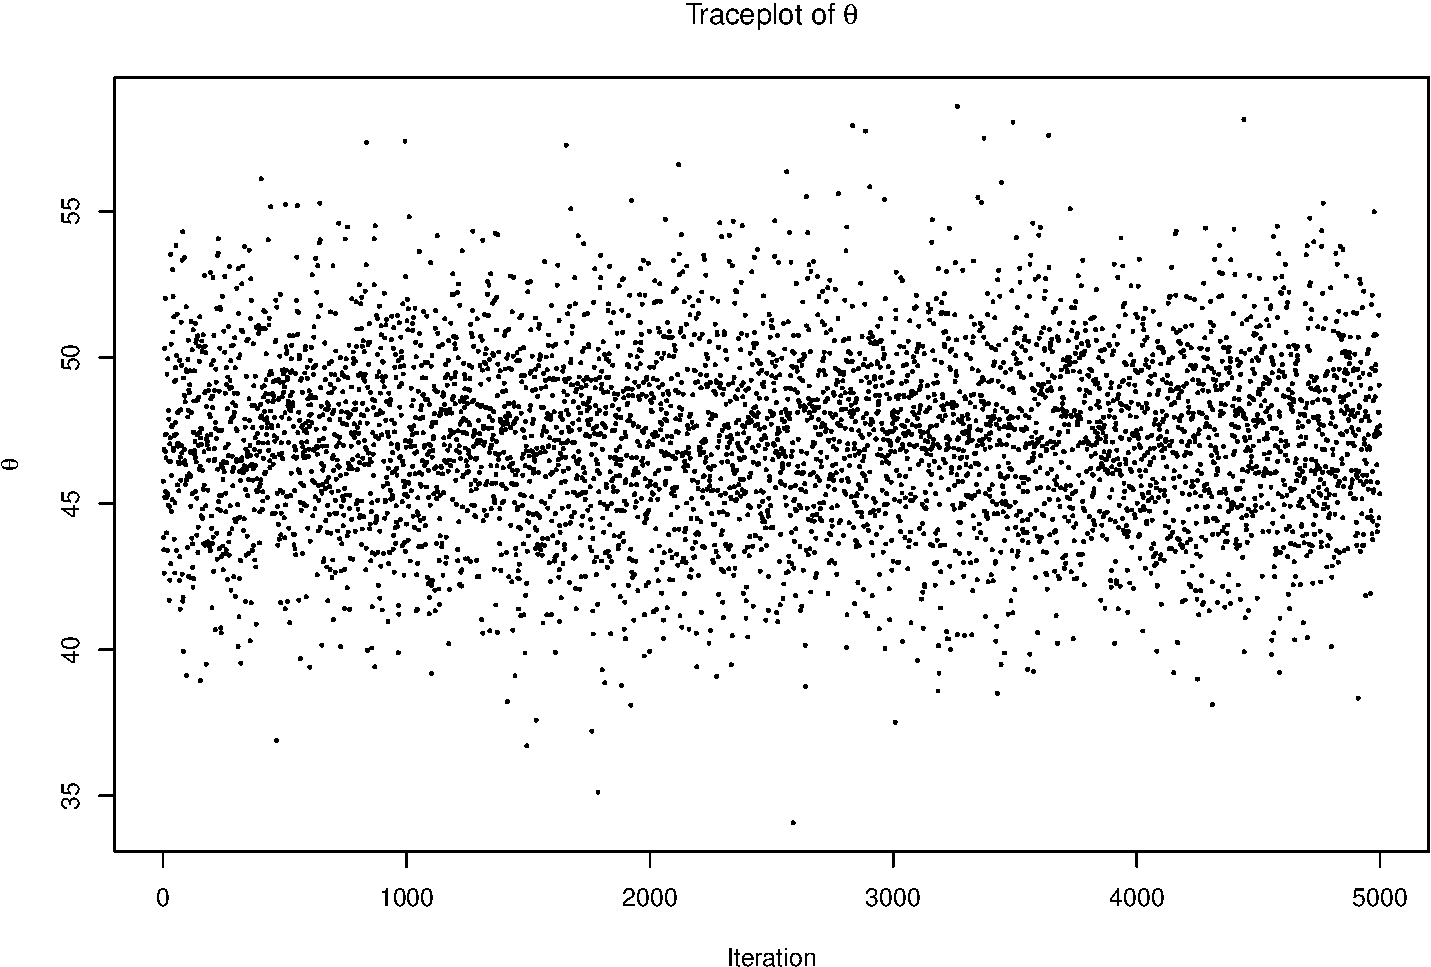
\includegraphics{08-multivariate-norm_files/figure-beamer/unnamed-chunk-12-1.pdf}

\end{frame}

\begin{frame}{Traceplot of \(\theta_2\)}
\protect\hypertarget{traceplot-of-theta_2}{}

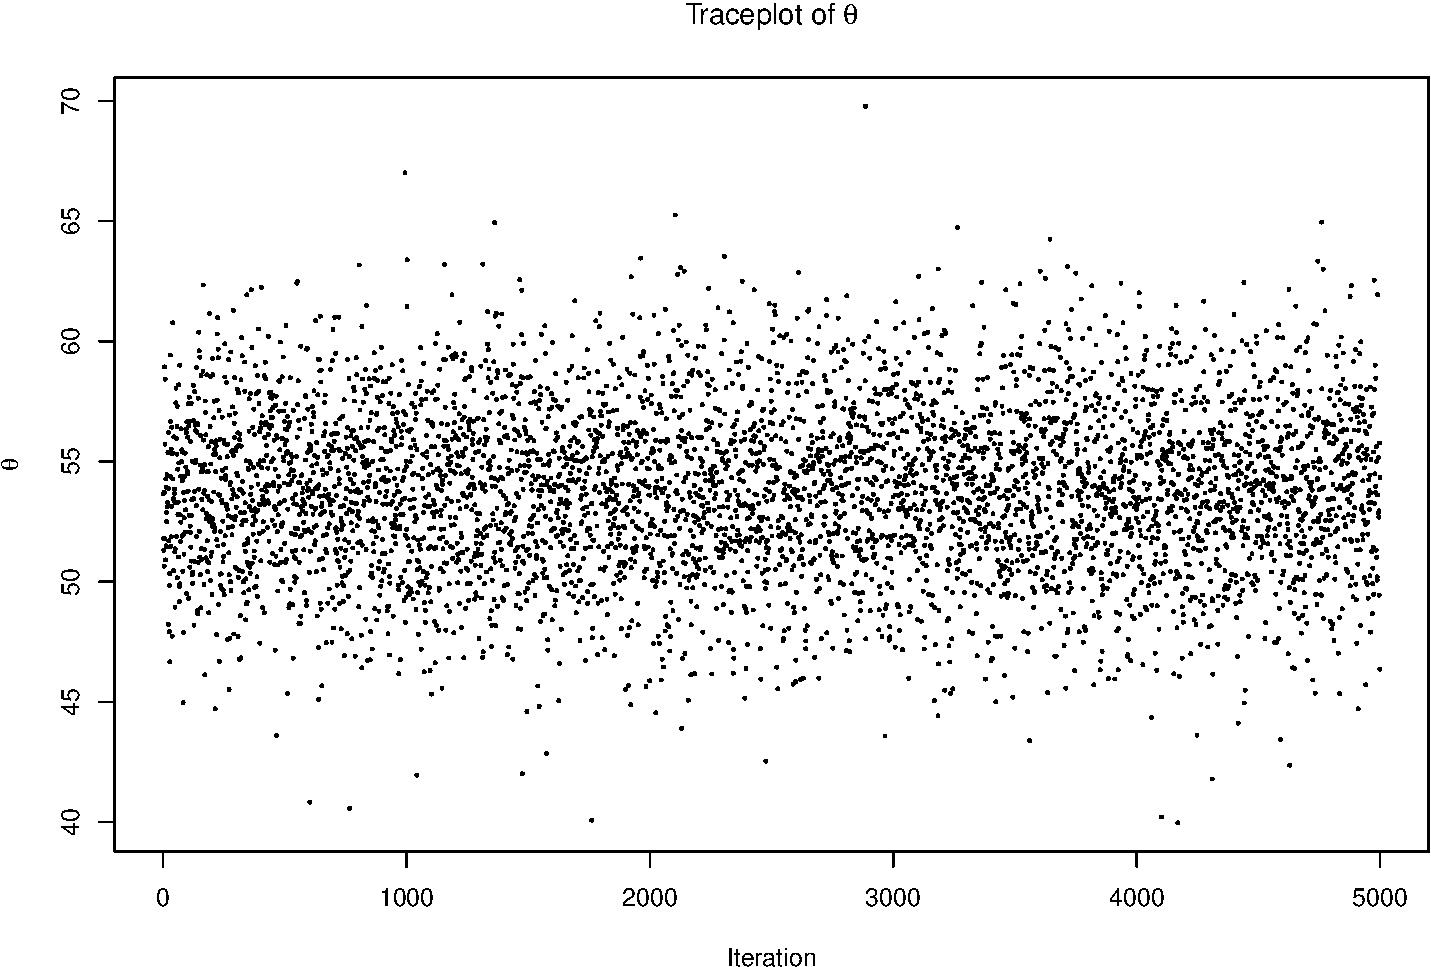
\includegraphics{08-multivariate-norm_files/figure-beamer/unnamed-chunk-13-1.pdf}

\end{frame}

\begin{frame}{Running average plot of \(\theta_1\)}
\protect\hypertarget{running-average-plot-of-theta_1}{}

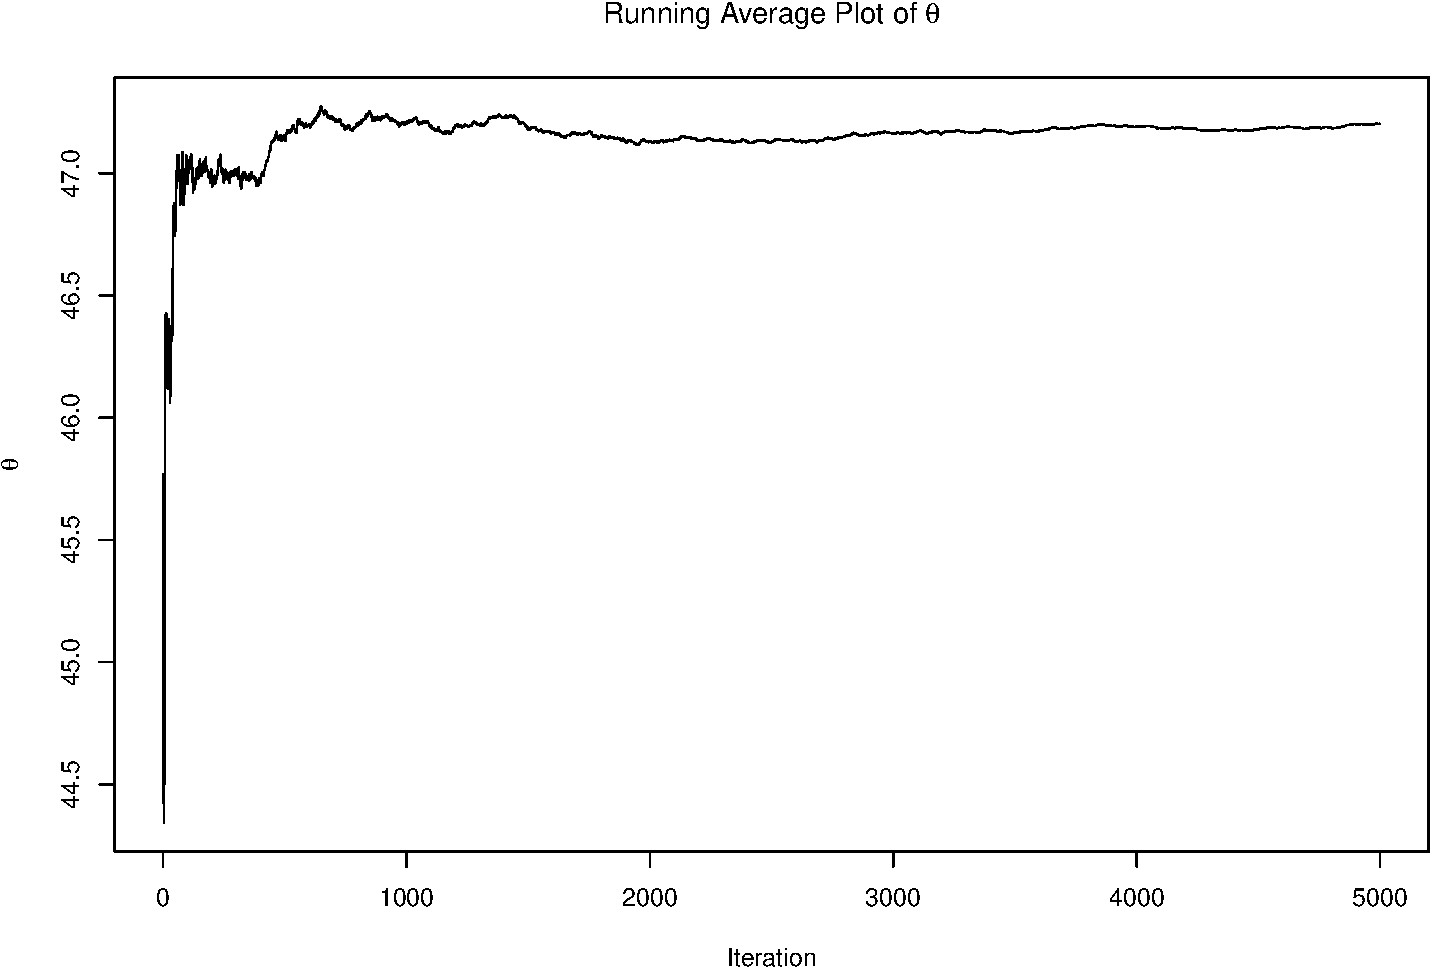
\includegraphics{08-multivariate-norm_files/figure-beamer/unnamed-chunk-14-1.pdf}

\end{frame}

\begin{frame}{Running average plot of \(\theta_2\)}
\protect\hypertarget{running-average-plot-of-theta_2}{}

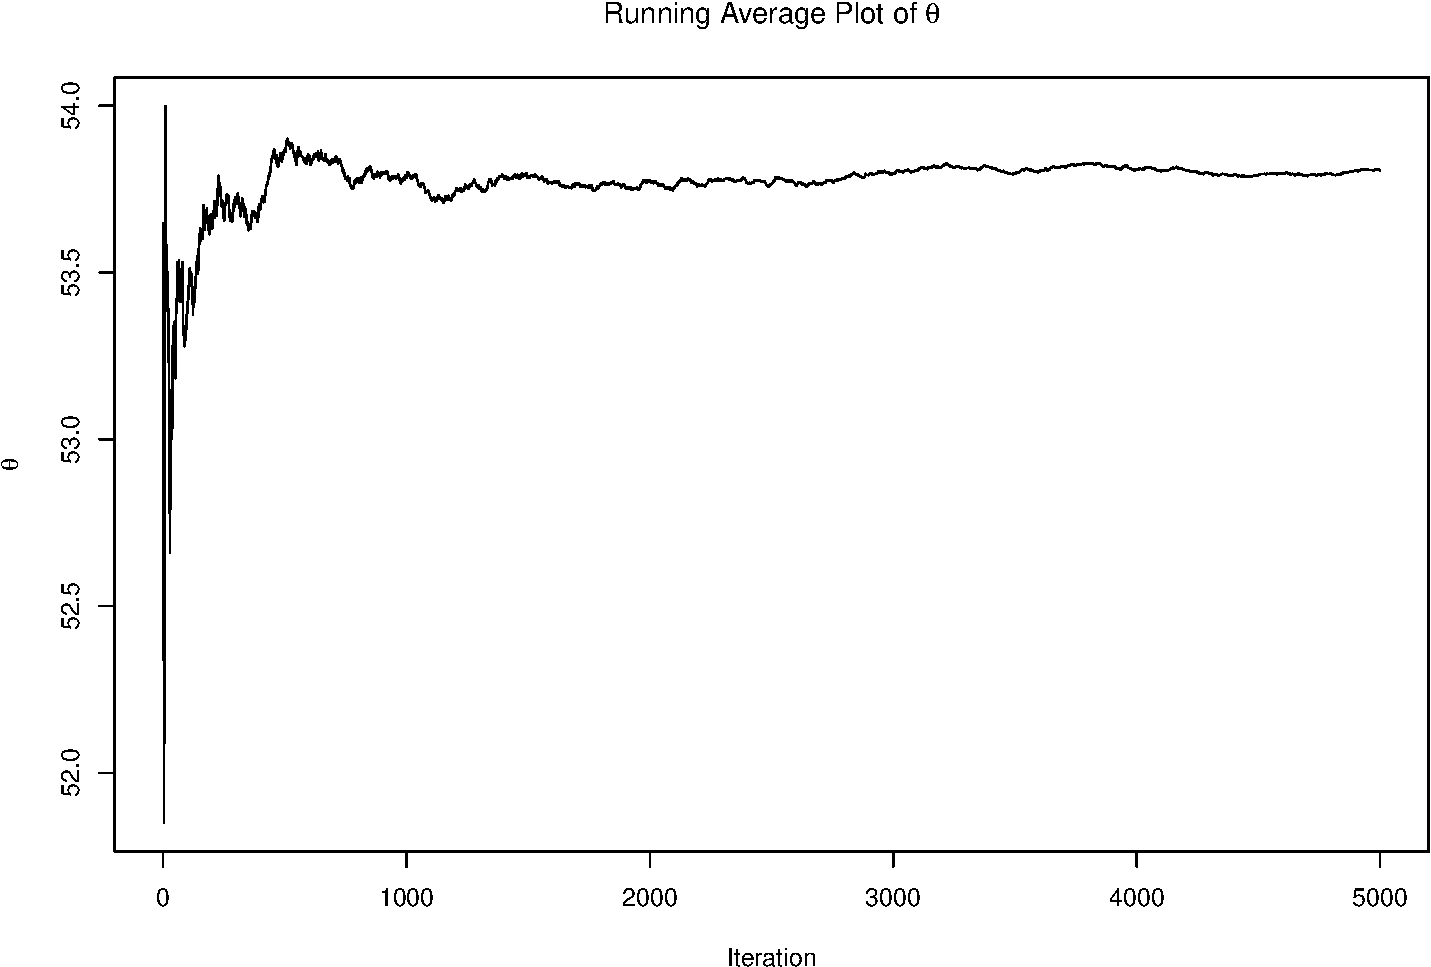
\includegraphics{08-multivariate-norm_files/figure-beamer/unnamed-chunk-15-1.pdf}

\end{frame}

\begin{frame}{Estimated density of \(\theta_1\)}
\protect\hypertarget{estimated-density-of-theta_1}{}

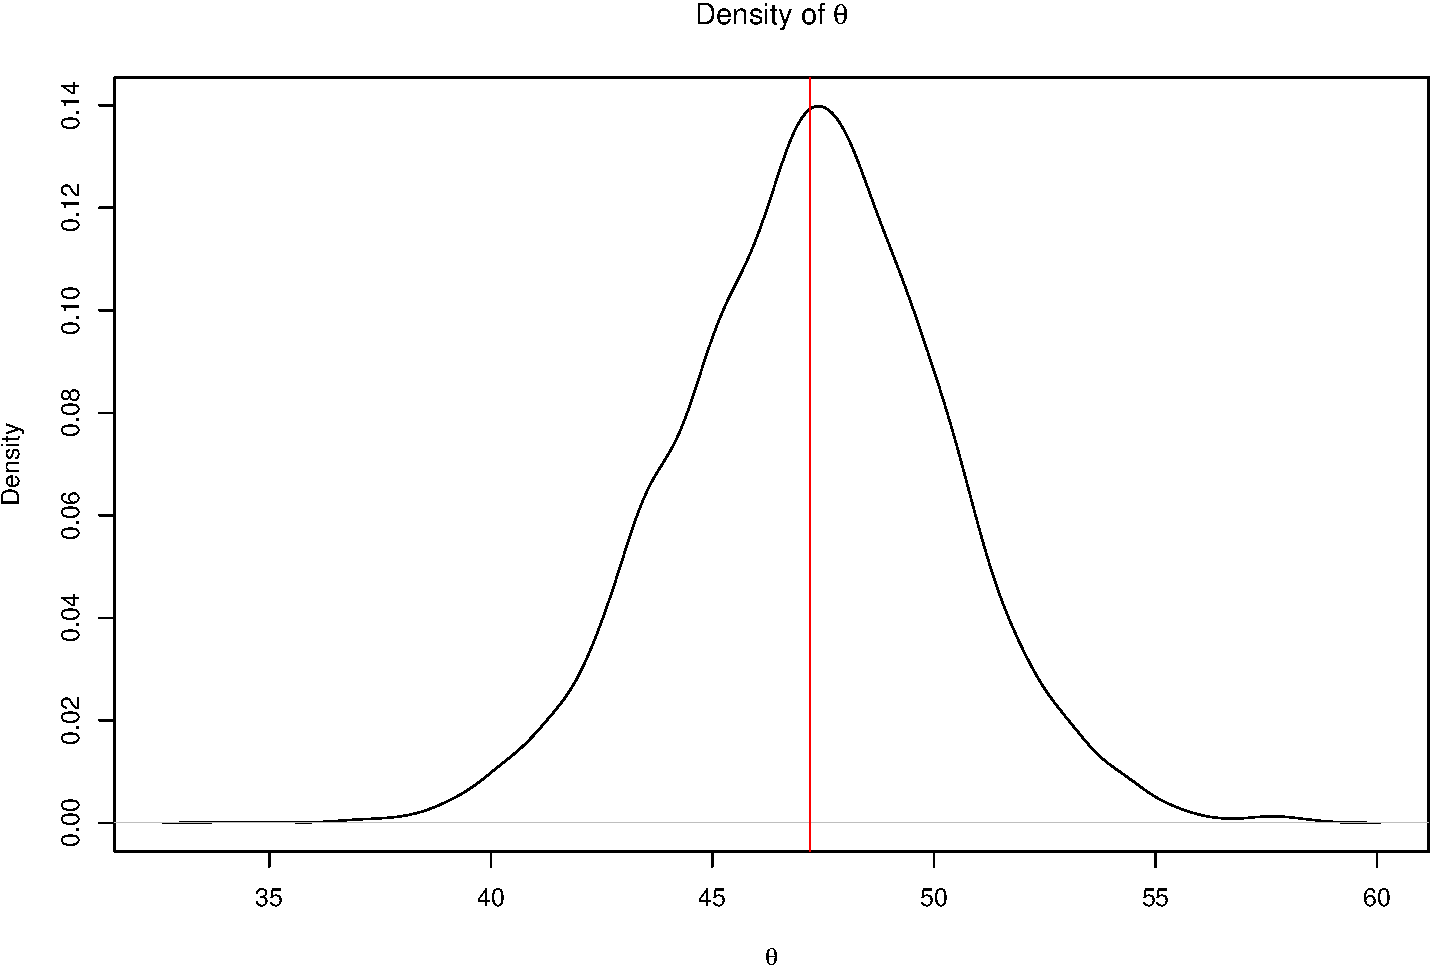
\includegraphics{08-multivariate-norm_files/figure-beamer/unnamed-chunk-16-1.pdf}

\end{frame}

\begin{frame}{Estimated density of \(\theta_2\)}
\protect\hypertarget{estimated-density-of-theta_2}{}

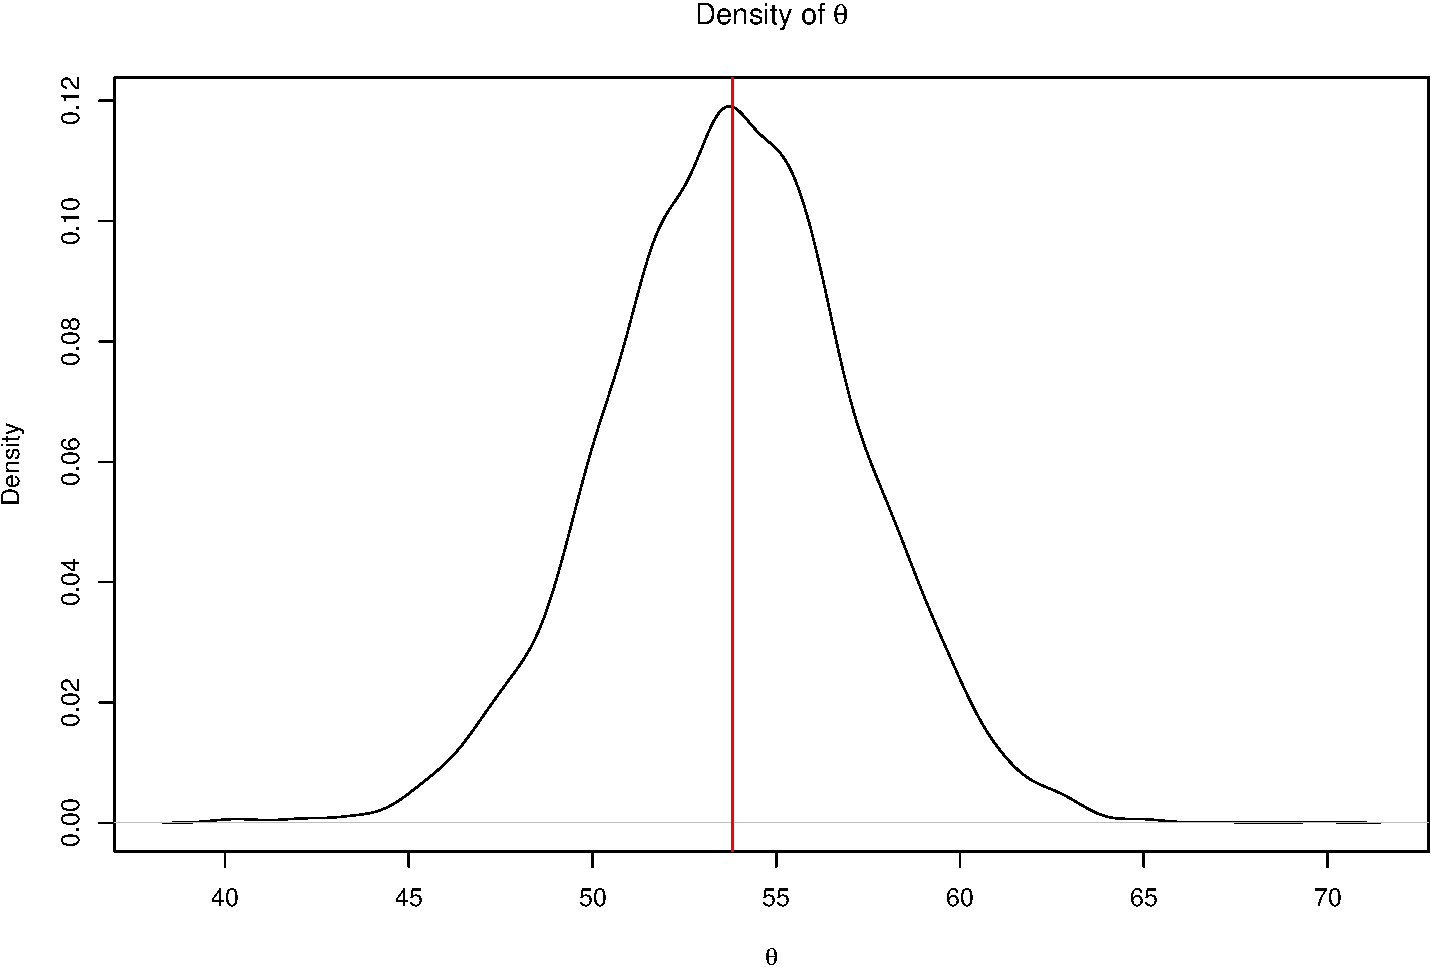
\includegraphics{08-multivariate-norm_files/figure-beamer/unnamed-chunk-17-1.pdf}

\end{frame}

\begin{frame}{Traceplots and running average plots}
\protect\hypertarget{traceplots-and-running-average-plots}{}

The traceplots don't tell us much of anything, so this is why we examine
the running average plots. Specifically, the traceplots indicate that
the chain has not failed to converged.

The running average plots indicate that the sampler appears to be mixing
well by 5,000 iterations and that the chain has not failed to converged.

\end{frame}

\begin{frame}{Traceplots and running average plots of \(\sigma\)}
\protect\hypertarget{traceplots-and-running-average-plots-of-sigma}{}

Examine the trace plots and running average plots of \(\Sigma\) on your
own.

\end{frame}

\begin{frame}{Return to posterior inference}
\protect\hypertarget{return-to-posterior-inference}{}

Given our samples from our Gibbs sampler, we can approximate posterior
probabilities and confidence regions.

\end{frame}

\begin{frame}[fragile]{Confidence regions}
\protect\hypertarget{confidence-regions}{}

\begin{Shaded}
\begin{Highlighting}[]
\KeywordTok{quantile}\NormalTok{(THETA[,}\DecValTok{2}\NormalTok{] }\OperatorTok{-}\StringTok{ }\NormalTok{THETA[,}\DecValTok{1}\NormalTok{], }\DataTypeTok{prob=}\KeywordTok{c}\NormalTok{(}\FloatTok{0.025}\NormalTok{,}\FloatTok{0.5}\NormalTok{,}\FloatTok{0.975}\NormalTok{))}
\end{Highlighting}
\end{Shaded}

\begin{verbatim}
##      2.5%       50%     97.5% 
##  1.356260  6.614818 11.667128
\end{verbatim}

\end{frame}

\begin{frame}[fragile]{Posterior inference}
\protect\hypertarget{posterior-inference-1}{}

Suppose we were to give the exams/instruction to a large population,
then would the average score on the second exam be higher than the first
second?

We can quanify this by calculating
\[Pr(\theta_2 > \theta_1 \mid y_1,\ldots y_n) = 0.99 
\]

\begin{Shaded}
\begin{Highlighting}[]
\KeywordTok{mean}\NormalTok{(THETA[,}\DecValTok{2}\NormalTok{] }\OperatorTok{>}\StringTok{ }\NormalTok{THETA[,}\DecValTok{1}\NormalTok{])}
\end{Highlighting}
\end{Shaded}

\begin{verbatim}
## [1] 0.9926
\end{verbatim}

\end{frame}

\begin{frame}{Detailed Takeaways on Background}
\protect\hypertarget{detailed-takeaways-on-background}{}

\begin{itemize}
\tightlist
\item
  Understanding vectors, matrices and notation\\
\item
  Understanding how to write multivariate notation for a conceptual
  problem
\item
  Understanding how to write general multivariate notation
\item
  Background on linear algebra
\item
  Determinants, traces, quadratic forms
\item
  Knowing how to do simple proofs such as the exercises from class
\end{itemize}

\end{frame}

\begin{frame}{Detailed Takeaways on Multivariate Normal Models}
\protect\hypertarget{detailed-takeaways-on-multivariate-normal-models}{}

\begin{itemize}
\tightlist
\item
  The multivariate normal distribution (MVN)
\item
  Exercise with the MVN
\item
  MVN-MVN semi-conjugacy
\item
  The inverse wishart distribution
\item
  MVN-inverse wishart semi-conjugacy
\item
  The MVN-MVN-inverse wishart model
\item
  Applying a Gibbs sampler
\item
  How to draw samples from the MVN and inverse wishart distributions
\item
  Case study on reading comprehension
\end{itemize}

\end{frame}

\begin{frame}{Proof of Lemma 1}
\protect\hypertarget{proof-of-lemma-1}{}

\[tr(AB) = tr(BA)\]

Proof: Suppose that \(A_{n \times n}\) and \(B_{n \times n}.\)

Recall that by definition \(tr(A) = \sum_{i=1}^n a_{ii}.\) By definition
\begin{align}
tr(AB) &= \sum_{i=1}^n (AB)_{ii} \\
& \sum_{i=1}^n \sum_{j=1}^n a_{ij} b_{ji}\\
& \sum_{i=1}^n \sum_{j=1}^n b_{ji} a_{ij} \\
&= \sum_{i=1}^n (BA)_{ii} 
= tr(BA)
\end{align}

\end{frame}

\begin{frame}{Exam II Preparation}
\protect\hypertarget{exam-ii-preparation}{}

Consider the following Exponential model for an observation \(x\):
\[ p(x|a,b) = a b \exp(- a b x) \I(x>0)\] and suppose the prior is
\[ p(a,b) = \exp(- a - b)\I(a,b>0). \]

\end{frame}

\begin{frame}{Exam II Preparation}
\protect\hypertarget{exam-ii-preparation-1}{}

\begin{enumerate}
\tightlist
\item
  Write out the \(p(a,b \mid x).\) Is is something you know how to
  sample from? Explain.
\item
  Derive any conditional distributions needed for a Gibbs sampler.
\item
  Write pseudo code to illustrate how one would utilize a Gibbs sampler
  to approximate the posterior distribution.
\end{enumerate}

\end{frame}

\begin{frame}{Solution}
\protect\hypertarget{solution}{}

\begin{enumerate}
\tightlist
\item
  The posterior distribution can be written as
\end{enumerate}

\begin{align}
p(a,b \mid x)
& = a b \exp(- a b x)  \times \exp(- a - b)\I(a,b,x>0)
\end{align}

This distribution is not something that appears to be a known
distribution or looks like it might be something easy to sample from,
thus, Gibbs sampling is a natural choice. (Metropolis could be used as
well.)

\end{frame}

\begin{frame}{Solution}
\protect\hypertarget{solution-1}{}

\begin{enumerate}
\setcounter{enumi}{1}
\tightlist
\item
  We must derive the full conditionals \(a \mid b,x\) and
  \(b \mid a,x.\) Consider
\end{enumerate}

\begin{align}
    p(a \mid b,x)
    &\underset{a}{\propto} p(x,a,b) \\
    &\underset{a}{\propto} a \exp(-a b x - a)\I(a>0)  \\
    &= a \exp(-(b x + 1)a)\I(a>0)\\
    &\underset{a}{\propto} \Ga(a\mid 2,\, b x + 1).
\end{align}

\end{frame}

\begin{frame}{Solution}
\protect\hypertarget{solution-2}{}

It follows that

\[p(b \mid a,x) {\propto} \Ga(b\mid 2,\, a x + 1).\]

\end{frame}

\begin{frame}{Solution}
\protect\hypertarget{solution-3}{}

Initialize \((a,b)\) to \((a_0, b_0).\)

\begin{enumerate}
\tightlist
\item
  For the first iteration of the Gibbs sampler,
\end{enumerate}

Draw \(a\) from \(a \mid b=b_0,x\)

Draw \(b\) from \(b \mid a=a_1,x\)

in order to get \((a_1,b_1).\)

\begin{enumerate}
\setcounter{enumi}{1}
\tightlist
\item
  For the second iteration of the Gibbs sampler,
\end{enumerate}

Draw \(a\) from \(a \mid b=b_1,x\)

Draw \(b\) from \(b \mid a=a_2,x\)

in order to get \((a_2,b_2).\)

M. For the \(M\)th iteration of the Gibbs sampler,

Draw \(a\) from \(a \mid b=b_{M-1},x\)

Draw \(b\) from \(b \mid a=a_{M},x\)

in order to get \((a_M,b_M).\)

\end{frame}

\end{document}
